\section{Results}
\label{sec:results}

The GeoSoil-Cuba workflow produced validated spatial
datasets, satellite-derived vegetation indices, and
statistical summaries describing soil-map coverage
and vegetation variability within the study area.

The results are organized into eight subsections
covering soil topology, spatial coverage, satellite
acquisition screening, preliminary NDVI inspection,
agricultural-region selection, temporal variability,
spatial NDVI distributions, and field-level observations.


\subsection{Soil Topology and Area-Accounting Validation}
\label{subsec:topology_validation}

The topology assessment identified differences between
the summed areas of individual clipped soil polygons
and the area of their geometric union. These
measurements were compared in the source coordinate
reference system (EPSG:3795) and after reprojection
to UTM Zone 17N (EPSG:32617).

In EPSG:3795, the sum of all clipped soil polygon
areas was 162.907~km$^2$, comprising
161.984~km$^2$ of classified soil polygons and
0.922~km$^2$ associated with an undefined
classification. The corresponding geometric union
covered 162.852~km$^2$, yielding a difference
of approximately 0.055~km$^2$.

After reprojection to EPSG:32617, the sum of all
polygon areas decreased to 162.820~km$^2$,
comprising 161.899~km$^2$ of classified soil
polygons and 0.922~km$^2$ associated with the
undefined classification. The geometric union
covered 162.766~km$^2$, again yielding a
difference of approximately 0.055~km$^2$.

The total polygon-area sum decreased by
0.086~km$^2$ (approximately 0.053\%)
between the two CRSs. The geometric union
area decreased by a similar amount, while
the difference between the polygon-area sum
and the geometric union remained nearly
unchanged. These results demonstrate the
sensitivity of planar area measurements to
coordinate reference system transformations,
while confirming that the overlap-related
area difference was consistent between
the two CRSs.

Pairwise intersection analysis identified
90 polygon pairs with positive-area overlaps.
Their cumulative pairwise overlap area was
0.054919~km$^2$, representing approximately
0.034\% of the summed polygon area in
EPSG:32617.

The largest individual overlap measured
0.046807~km$^2$ and occurred between
Aluvial Poco Diferenciado (2618) and
Pardo con Carbonatos Típico (1001).

The principal area-accounting and topology
results are summarized in
\Cref{tab:soil_topology_validation}.

\begin{table}[htbp]
	\centering
	\caption{
		Soil polygon area accounting and
		topology validation results.
	}
	\label{tab:soil_topology_validation}
	\small
	
	\begin{tabular}{lr}
		\hline
		\textbf{Metric} & \textbf{Value} \\
		\hline
		
		\multicolumn{2}{l}{
			\textit{Area measurements in EPSG:3795}
		} \\
		\hline
		
		Classified soil polygon-area sum (km$^2$)
		& 161.984 \\
		
		Undefined soil polygon area (km$^2$)
		& 0.922 \\
		
		Total polygon-area sum (km$^2$)
		& 162.907 \\
		
		Geometric union area (km$^2$)
		& 162.852 \\
		
		Sum minus union (km$^2$)
		& 0.055 \\
		
		\hline
		\multicolumn{2}{l}{
			\textit{Area measurements in EPSG:32617}
		} \\
		\hline
		
		Classified soil polygon-area sum (km$^2$)
		& 161.899 \\
		
		Undefined soil polygon area (km$^2$)
		& 0.922 \\
		
		Total polygon-area sum (km$^2$)
		& 162.820 \\
		
		Geometric union area (km$^2$)
		& 162.766 \\
		
		Sum minus union (km$^2$)
		& 0.055 \\
		
		\hline
		\multicolumn{2}{l}{
			\textit{CRS comparison}
		} \\
		\hline
		
		Change in polygon-area sum (km$^2$)
		& $-0.086$ \\
		
		Relative change in polygon-area sum (\%)
		& $-0.053$ \\
		
		\hline
		\multicolumn{2}{l}{
			\textit{Topology validation}
		} \\
		\hline
		
		Overlapping polygon pairs
		& 90 \\
		
		Total pairwise overlap area (km$^2$)
		& 0.054919 \\
		
		Largest individual overlap (km$^2$)
		& 0.046807 \\
		
		Pairwise overlap / total polygon area (\%)
		& 0.034 \\
		
		\hline
	\end{tabular}
\end{table}

The cumulative pairwise overlap area closely
matched the difference between the summed
polygon areas and their geometric union in
EPSG:32617. Specifically, the sum-minus-union
difference was 0.054919~km$^2$, matching the
reported cumulative pairwise overlap area
to six decimal places.

However, pairwise overlap calculations may
count the same location more than once where
three or more polygons intersect. Consequently,
the cumulative pairwise overlap area should
not be interpreted as an exact measure of
the geographic area affected by overlaps.
Likewise, the difference between the polygon-area
sum and the geometric union represents excess
area arising from overlapping polygons rather
than necessarily the unique geographic extent
of the overlapping regions.

The detected overlaps were retained as
data-quality findings. No source soil-unit
boundaries were modified or removed to
eliminate these intersections.

\subsection{Soil and Vegetation Spatial Coverage}
\label{subsec:spatial_results}

The Area of Interest (AOI) covers approximately
178.47~km$^2$. The spatial coverage assessment
reported soil-map coverage of approximately
162.85~km$^2$, equivalent to 91.25\% of the AOI.

The corresponding uncovered area was
15.62~km$^2$, representing approximately
8.75\% of the AOI.

Water bodies occupied approximately
14.49~km$^2$ within the AOI. Of this area,
approximately 3.07~km$^2$ overlapped
existing soil polygons, while
11.42~km$^2$ was not covered by the
soil dataset.

The remaining non-water gaps accounted for
approximately 4.20~km$^2$, equivalent
to 2.35\% of the AOI.

The principal spatial coverage measurements
are presented in \Cref{tab:spatial_coverage}.

\begin{table}[htbp]
	\centering
	\caption{
		Reported spatial coverage of soil,
		water-body, and vegetation datasets
		within the Area of Interest.
	}
	\label{tab:spatial_coverage}
	
	\begin{tabular}{lrr}
		\hline
		
		\textbf{Spatial component} &
		\textbf{Area (km$^2$)} &
		\textbf{AOI (\%)} \\
		
		\hline
		
		Area of Interest
		& 178.47 & 100.00 \\
		
		Soil-map coverage
		& 162.85 & 91.25 \\
		
		Total soil-data gap
		& 15.62 & 8.75 \\
		
		Water-body area
		& 14.49 & 8.12 \\
		
		Water area not covered by soil polygons
		& 11.42 & 6.40 \\
		
		Remaining non-water gaps
		& 4.20 & 2.35 \\
		
		Vegetation coverage
		& 161.93 & 90.73 \\
		
		\hline
	\end{tabular}
\end{table}

The soil-map coverage reported in
\Cref{tab:spatial_coverage} differs slightly
from the geometric union area reported in
\Cref{tab:soil_topology_validation}.

The two measurements are therefore retained
as distinct reported results. Their difference
requires verification against the processing
stages and geometry sets used to calculate
the respective areas.

The spatial distribution of the remaining
soil-data gaps is shown in
\Cref{fig:remaining_soil_gaps}.

\begin{figure}[htbp]
	\centering
	
	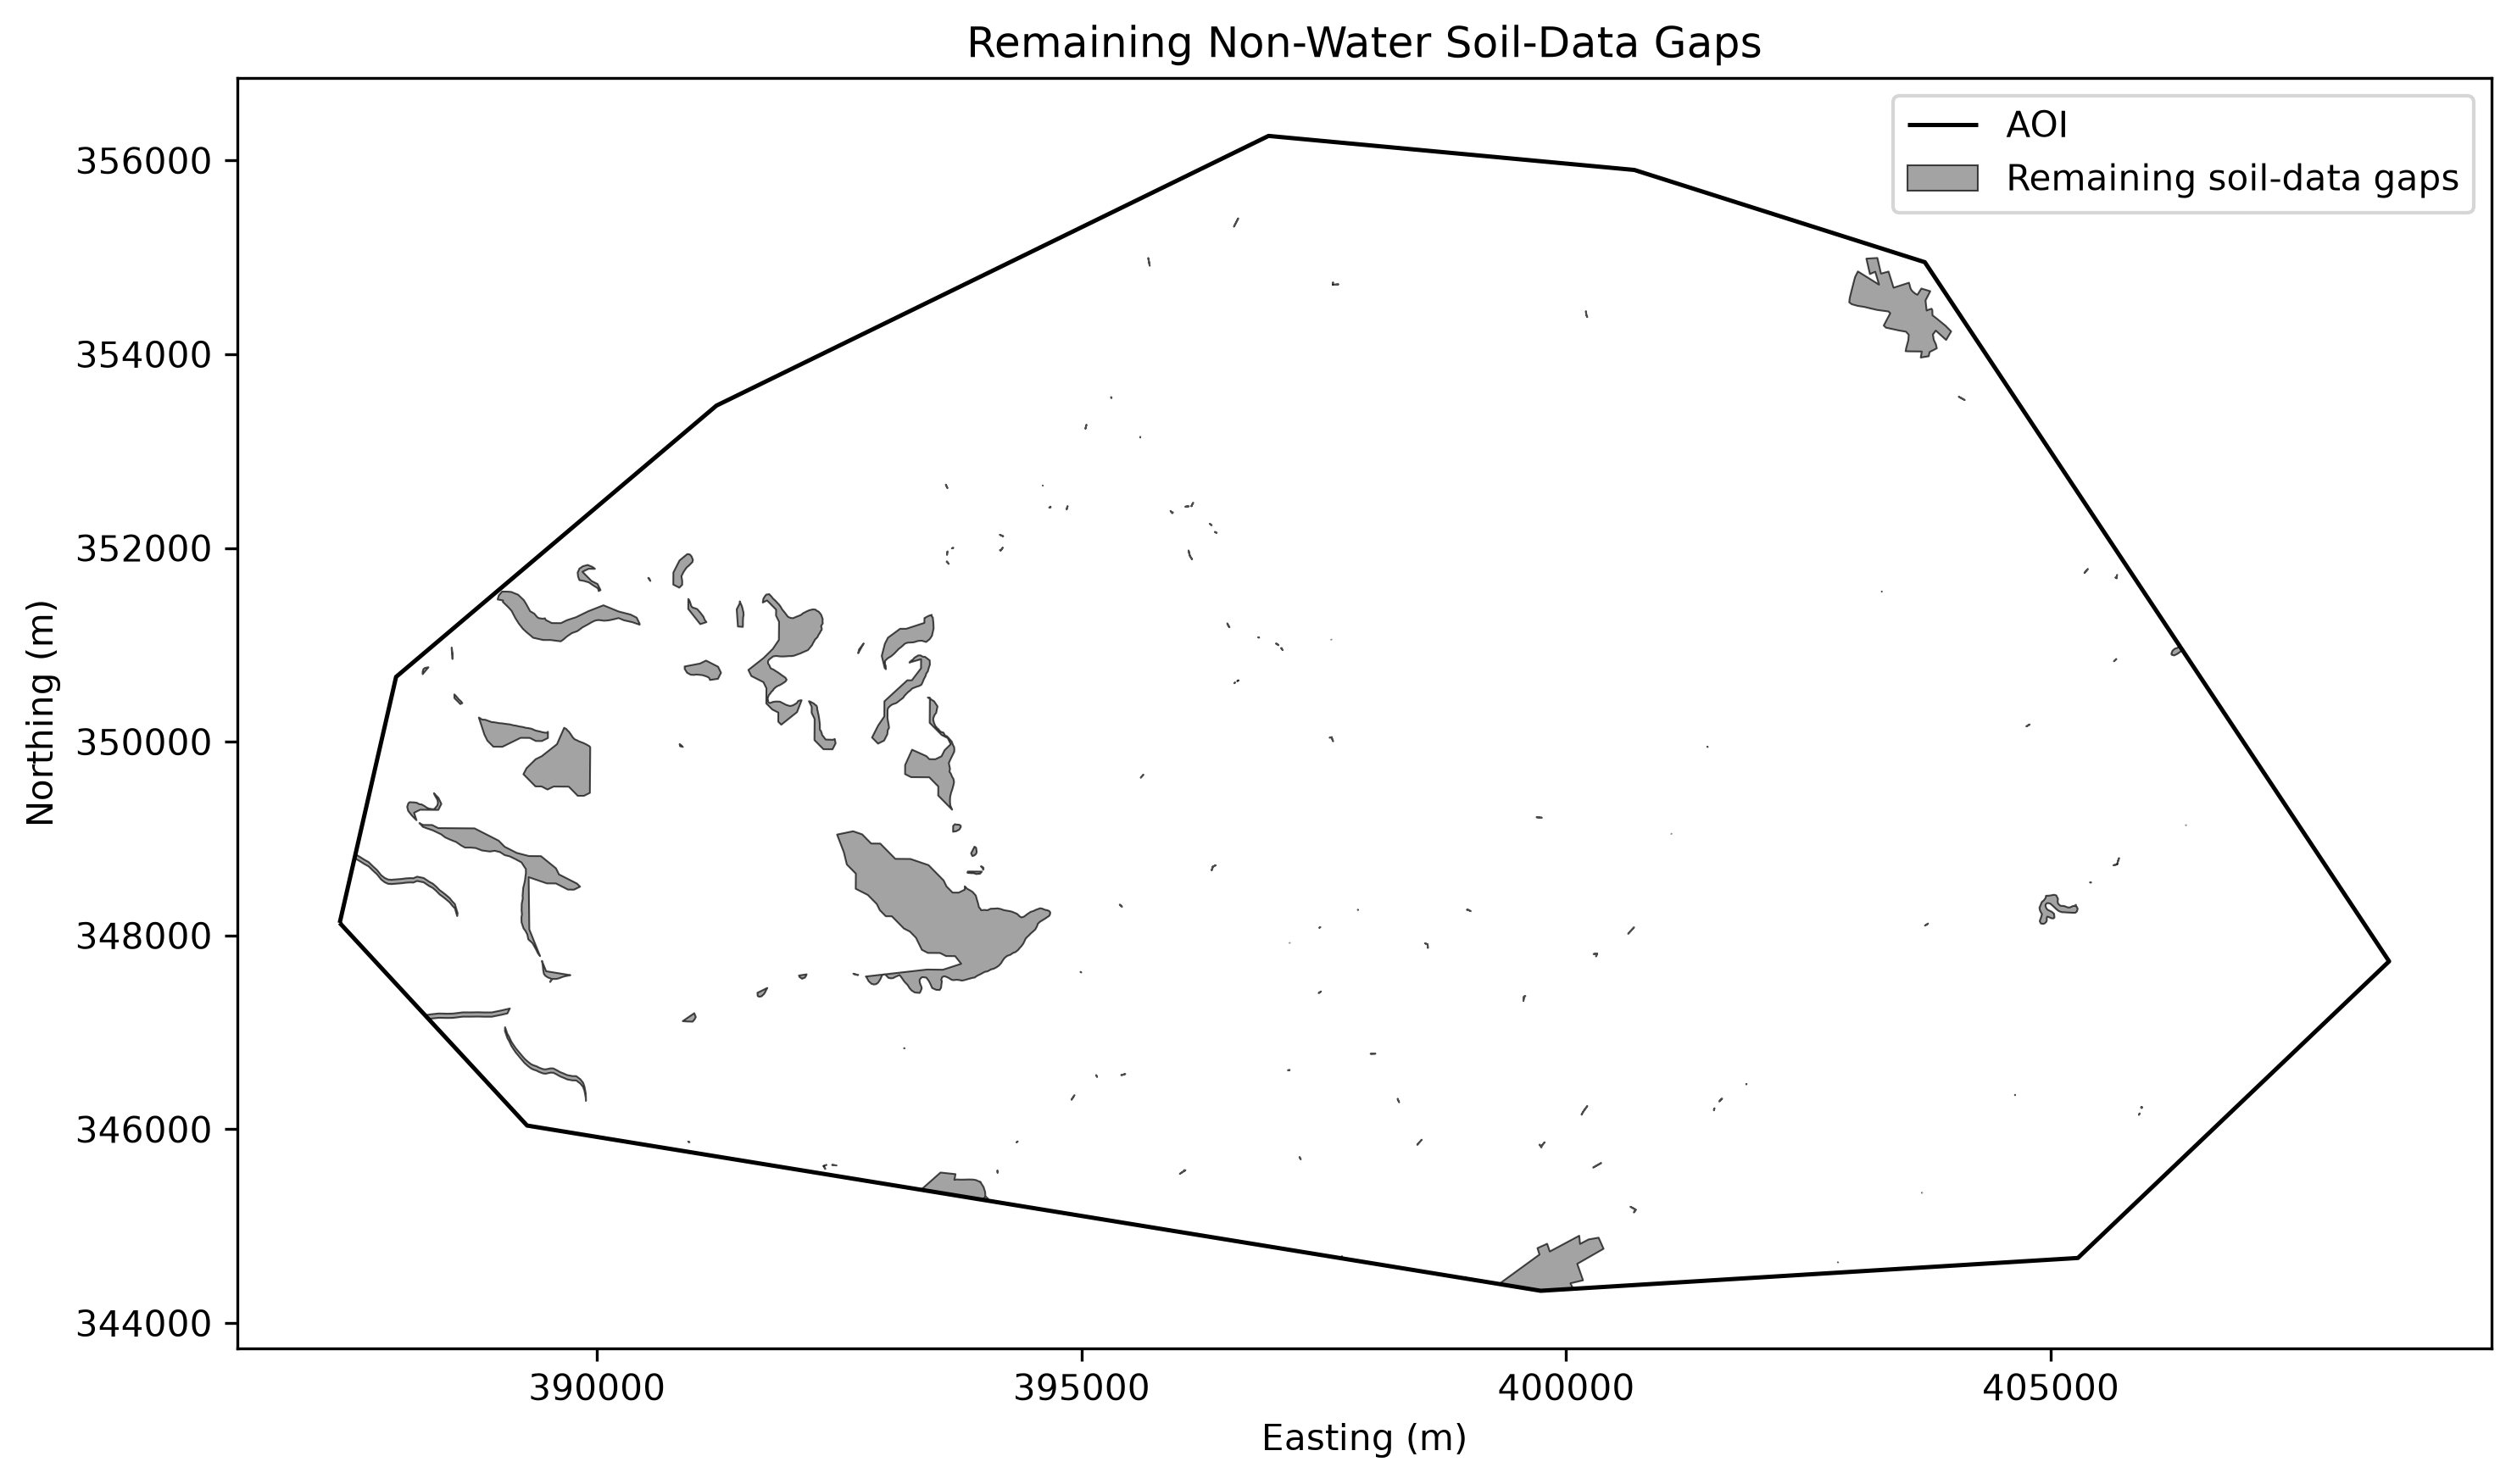
\includegraphics[
	width=0.90\linewidth
	]{../figures/remaining_soil_data_gaps.png}
	
	\caption{
		Spatial distribution of remaining
		areas without soil-map coverage
		within the AOI, following the
		identification of water-related
		gaps associated with the
		Mampostón reservoir.
	}
	
	\label{fig:remaining_soil_gaps}
\end{figure}

The clipped soil inventory contained one
polygon with the attribute combination
\texttt{Cód\_tipo = 0} and
\texttt{Cód\_stipo = 0}.

Because code zero was not defined as a
valid soil type or subtype in Anexo~6,
the polygon was classified as undefined
rather than assigned to an unsupported
soil category.

This polygon accounted for
0.922~km$^2$ of the summed soil
polygon area.

The spatial distribution of the mapped
soil units is presented in
\Cref{fig:soil_vegetation}.

\begin{figure}[htbp]
	\centering
	
	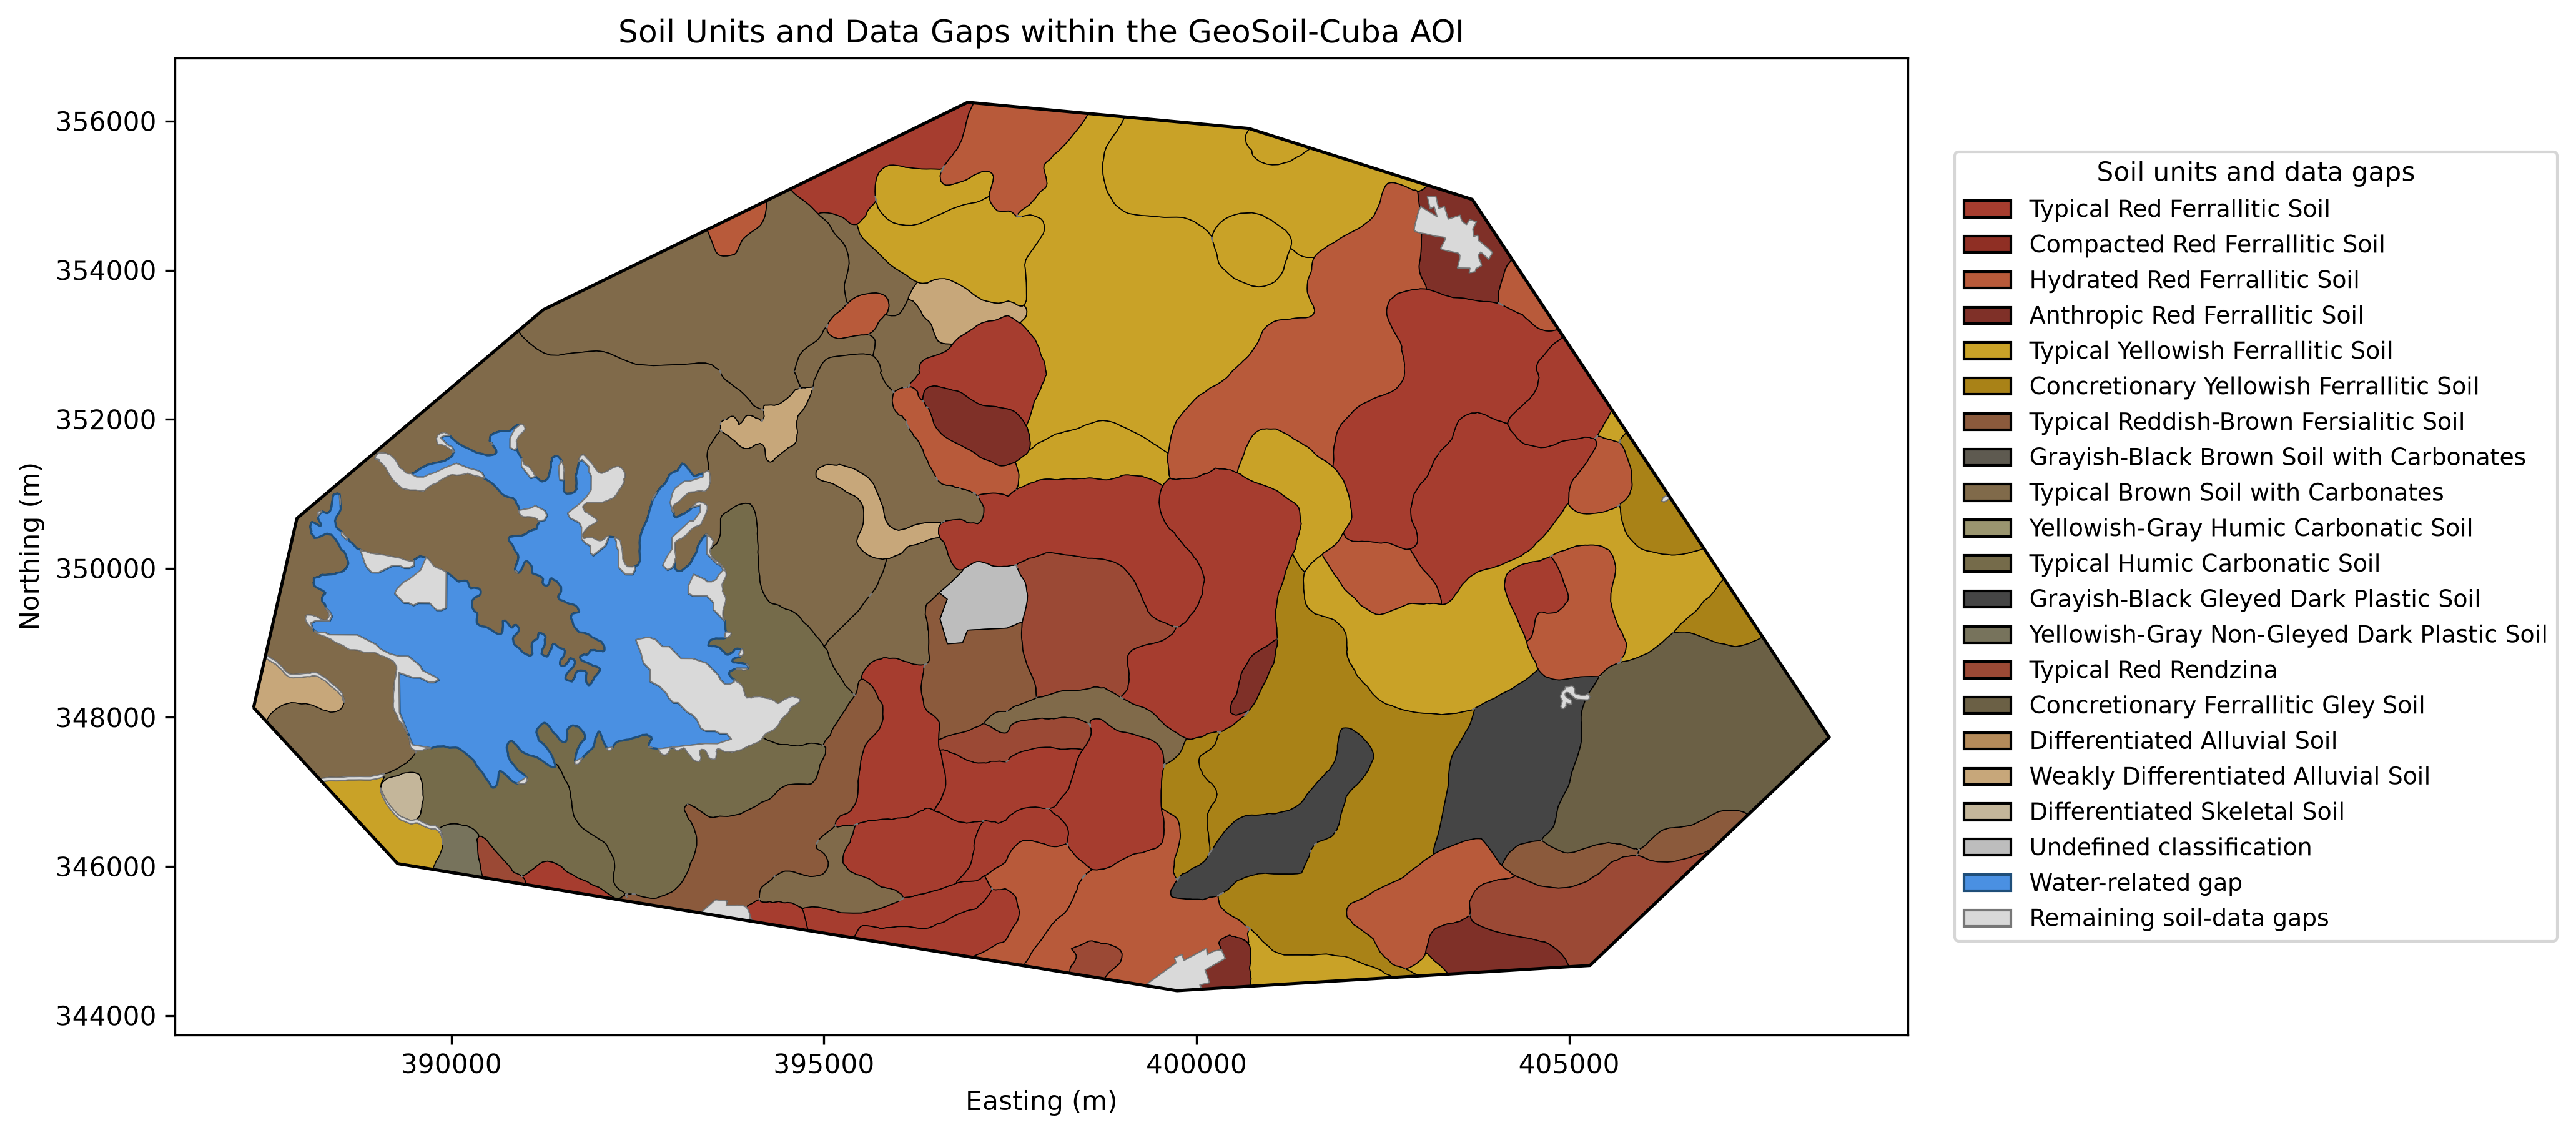
\includegraphics[
	width=\linewidth
	]{../figures/soil_units_aoi.png}
	
	\caption{
		Spatial distribution of mapped
		soil units within the AOI,
		including areas with undefined
		soil classification.
	}
	
	\label{fig:soil_vegetation}
\end{figure}

The vegetation and land-cover dataset
provided reported spatial coverage of
approximately 161.93~km$^2$.

The inventory included grasslands
(87.45~km$^2$), cultivated land
(75.86~km$^2$), secondary vegetation
(13.69~km$^2$), and flooded hydromorphic
areas (1.47~km$^2$).

The sum of these reported class areas
exceeds the stated vegetation coverage.
Consequently, these measurements cannot
be interpreted as a mutually exclusive
partition of the vegetation-covered area
without further verification of the
classification and area-accounting methods.

The spatial distribution of the vegetation
categories is illustrated in
\Cref{fig:vegetation_types}.

\begin{figure}[htbp]
	\centering
	
	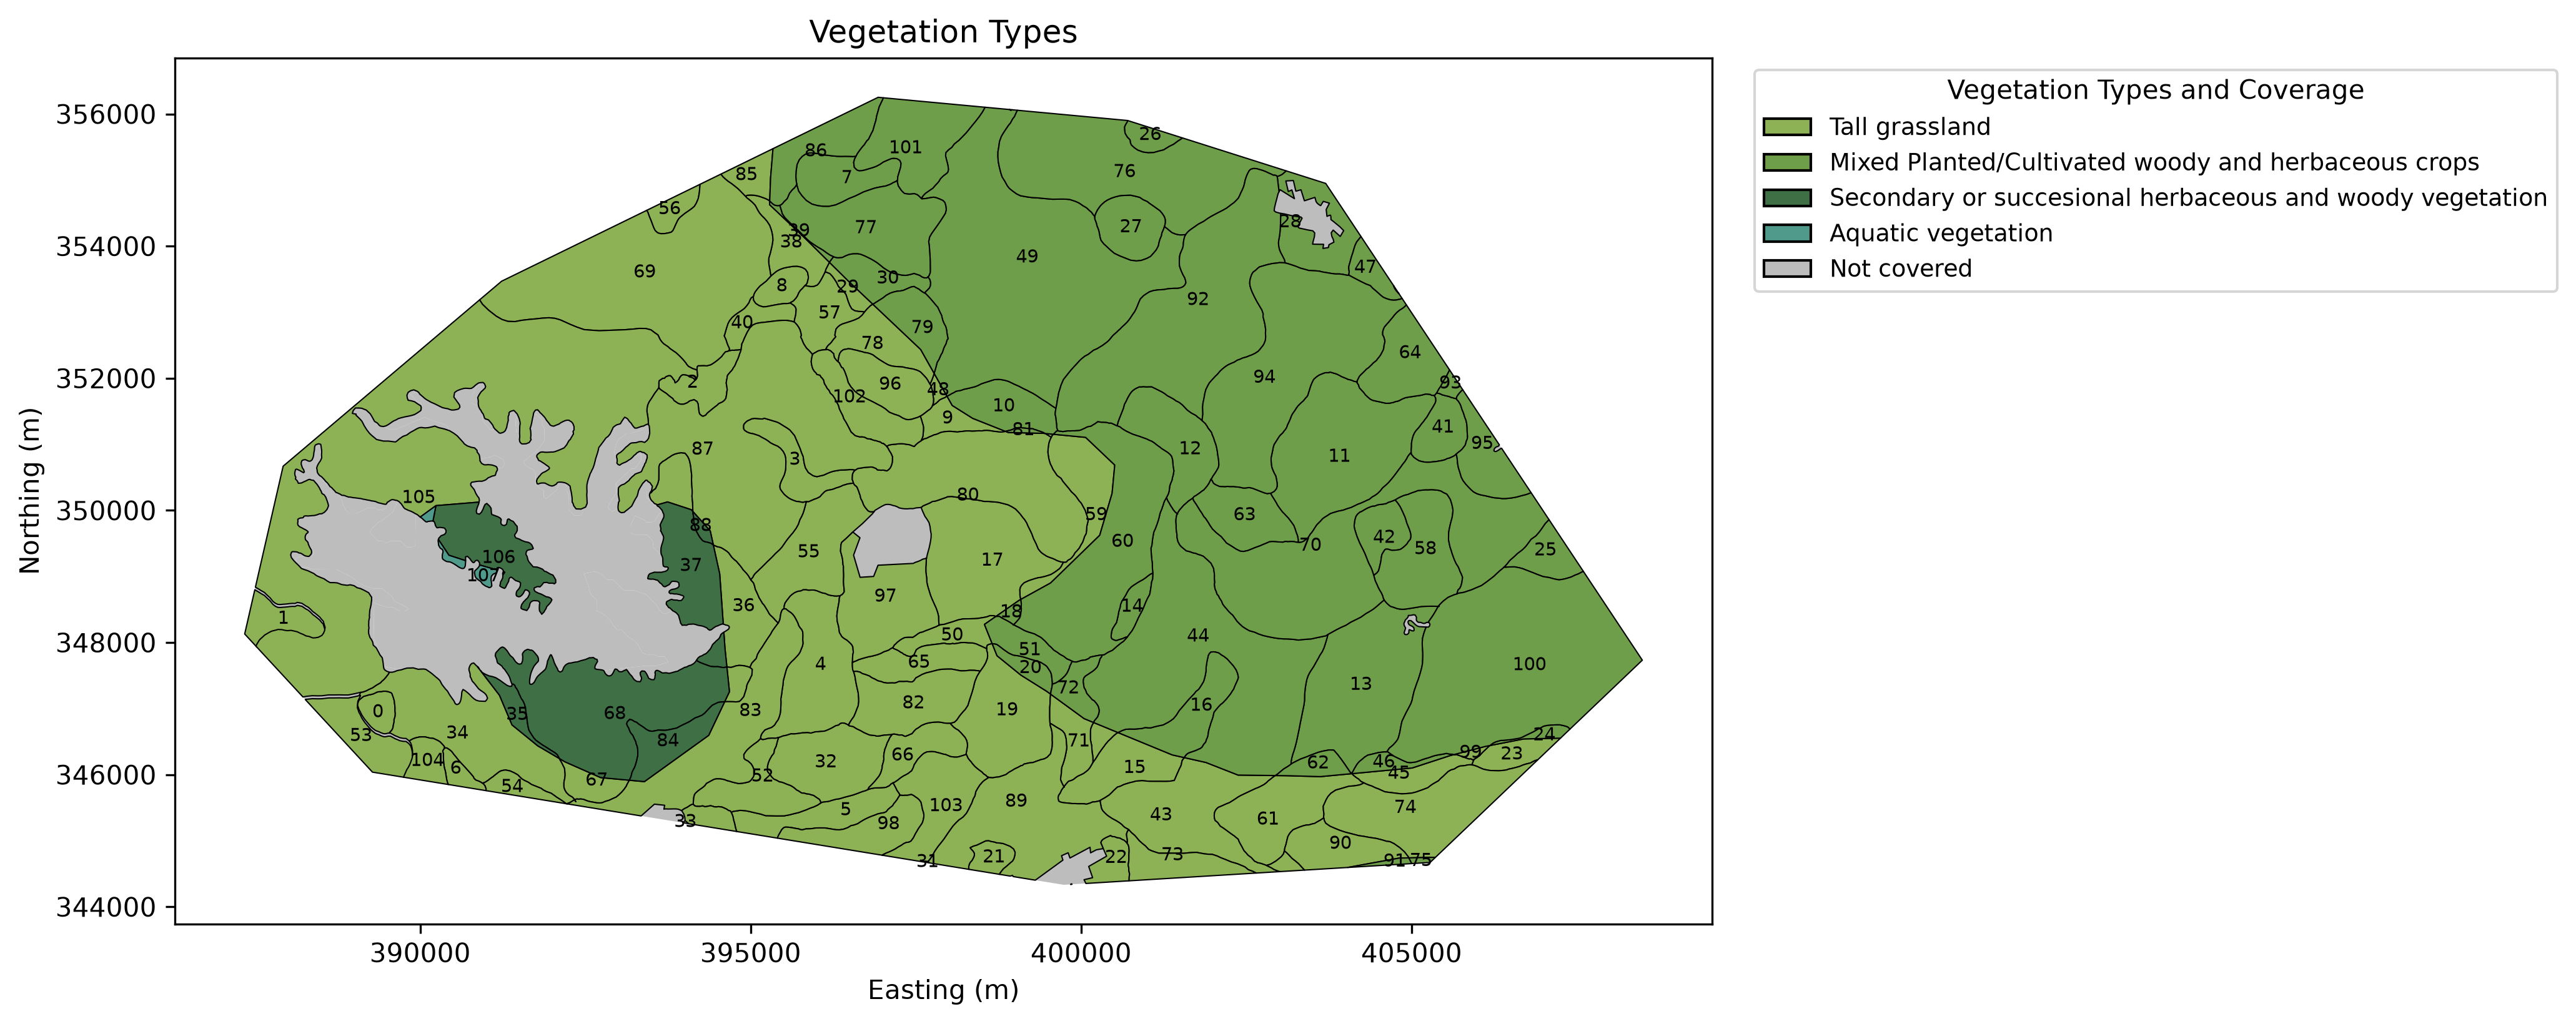
\includegraphics[
	width=\linewidth
	]{../figures/vegetation_types.png}
	
	\caption{
		Spatial distribution of mapped
		vegetation and land-cover
		categories within the AOI.
	}
	
	\label{fig:vegetation_types}
\end{figure}

These spatial datasets provided the basis
for integrating soil classifications with
existing vegetation and land-cover
information.


\subsection{Sentinel-2 Acquisition and Quality Screening}
\label{subsec:sentinel_results}

The Sentinel-2 inventory contained
226 observations acquired between
November 2025 and June 2026.

The mean catalogue-reported cloud-cover
percentage was 40.04\%, indicating
substantial variation in acquisition
conditions across the available imagery.

Following satellite processing,
32 NDVI rasters were generated for
the selected agricultural region.

The regional quality-screening procedure
retained 15 acquisitions with less
than 10\% cloud coverage within the
analysis region.

The accepted observations spanned
3 November 2025 to 16 June 2026.

The temporal distribution of these
acquisitions was not uniform, reflecting
the availability of observations meeting
the regional screening criterion.

Fourteen retained rasters contained
162,195 valid NDVI pixels, while one
contained 162,193 valid pixels.

The nearly constant valid-pixel counts
indicate that the accepted rasters
represented a stable spatial sampling
extent, although this numerical
consistency does not independently
establish the absence of residual
cloud or shadow contamination.


\subsection{Initial Inspection of NDVI Data}
\label{subsec:initial_ndvi_inspection}

A preliminary inspection was conducted
using 14 NDVI rasters from the available
Sentinel-2 observations.

The initial analysis examined spatial
NDVI patterns, temporal changes in
summary statistics, and differences
in pixel-level distributions.

A representative NDVI map from
3 November 2025 is presented in
\Cref{fig:initial_ndvi_map}.

\begin{figure}[htbp]
	\centering
	
	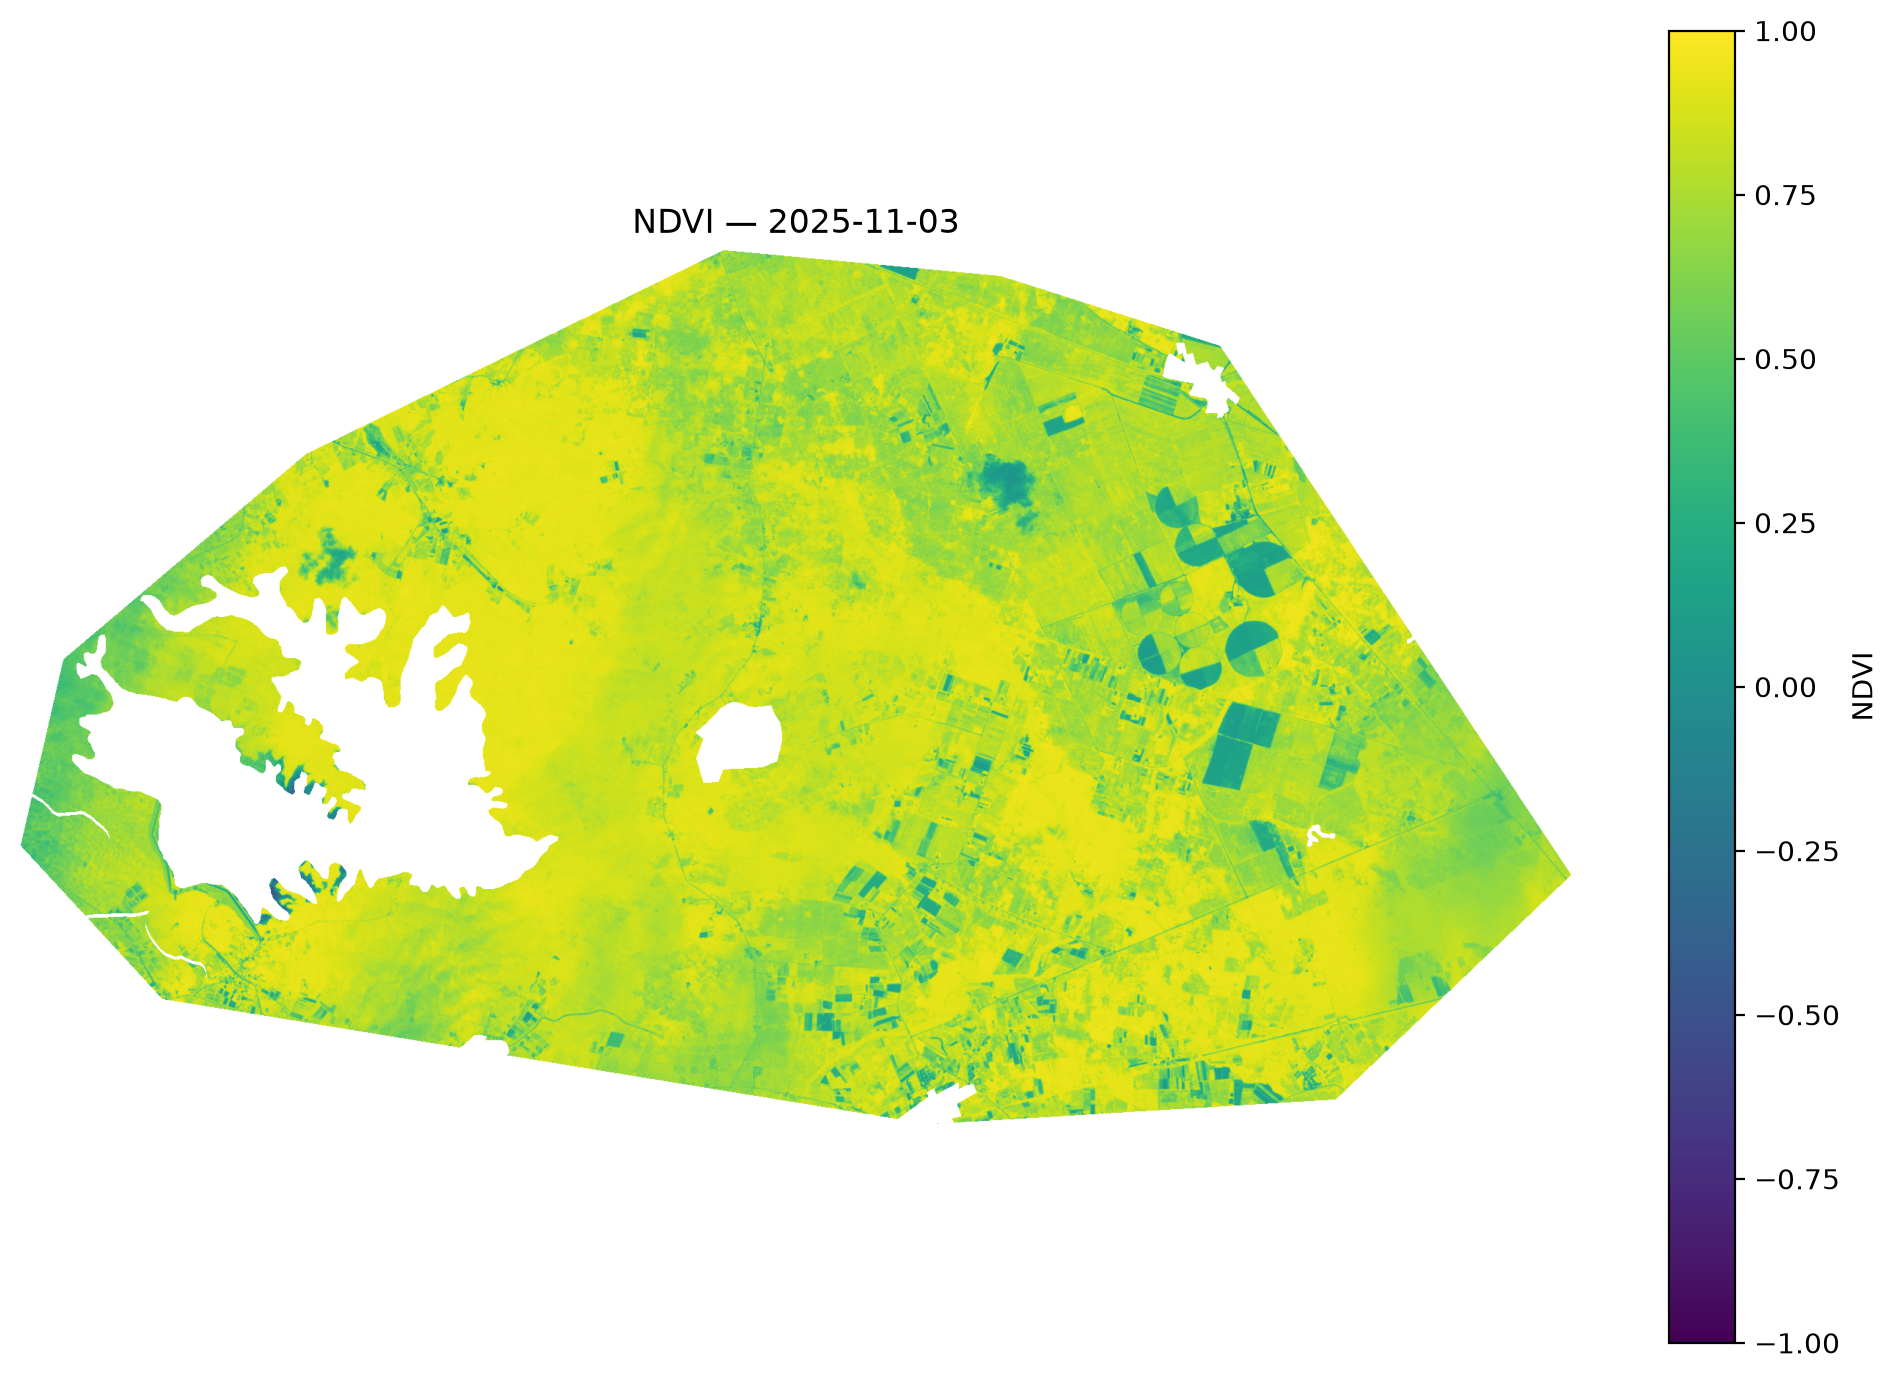
\includegraphics[
	width=0.90\linewidth
	]{../figures/stage5_figure_23.png}
	
	\caption{
		Preliminary NDVI map derived
		from Sentinel-2 imagery acquired
		on 3 November 2025.
	}
	
	\label{fig:initial_ndvi_map}
\end{figure}

The initial temporal summaries are
shown in \Cref{fig:initial_ndvi_timeseries},
while the corresponding pixel-level
distributions are presented in
\Cref{fig:initial_ndvi_boxplots}.

\begin{figure}[htbp]
	\centering
	
	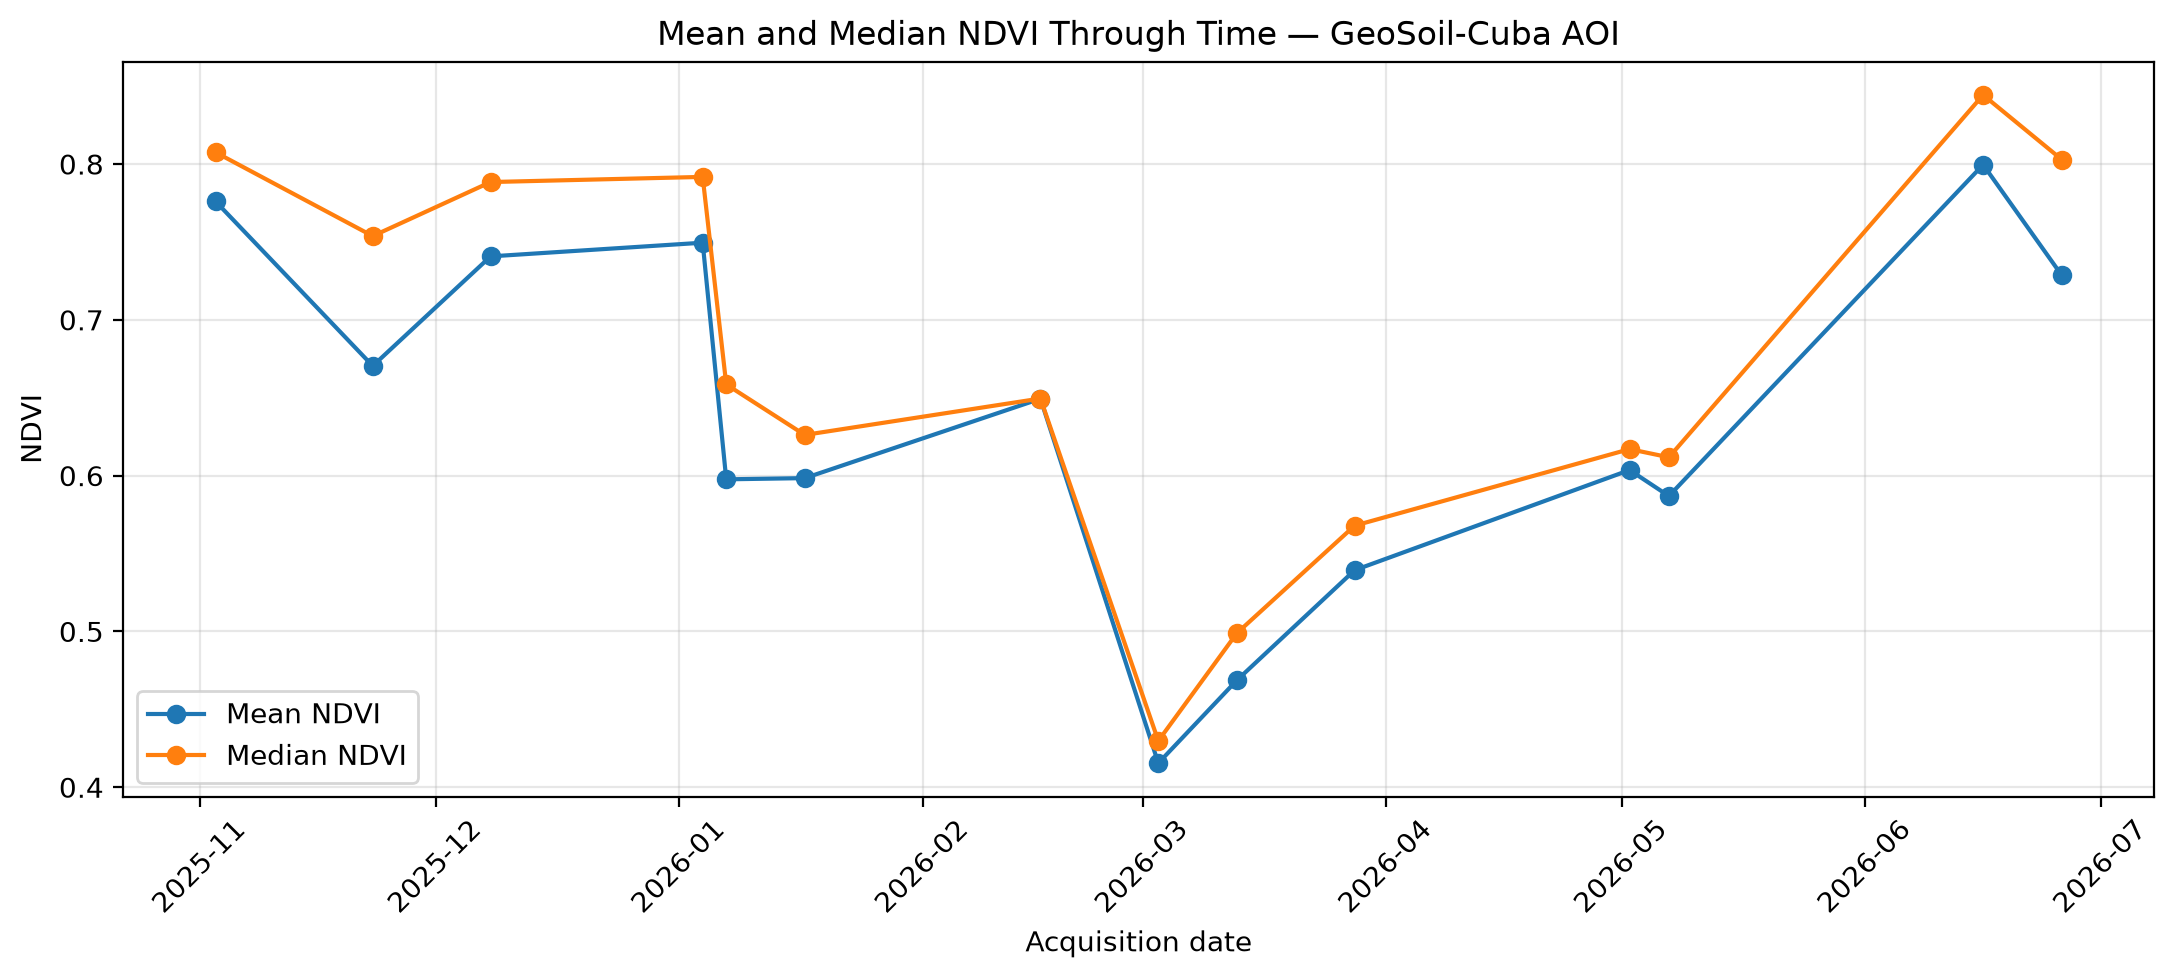
\includegraphics[
	width=0.90\linewidth
	]{../figures/stage5_figure_17.png}
	
	\caption{
		Preliminary temporal variation
		in mean and median NDVI across
		the initially selected raster
		observations.
	}
	
	\label{fig:initial_ndvi_timeseries}
\end{figure}

\begin{figure}[htbp]
	\centering
	
	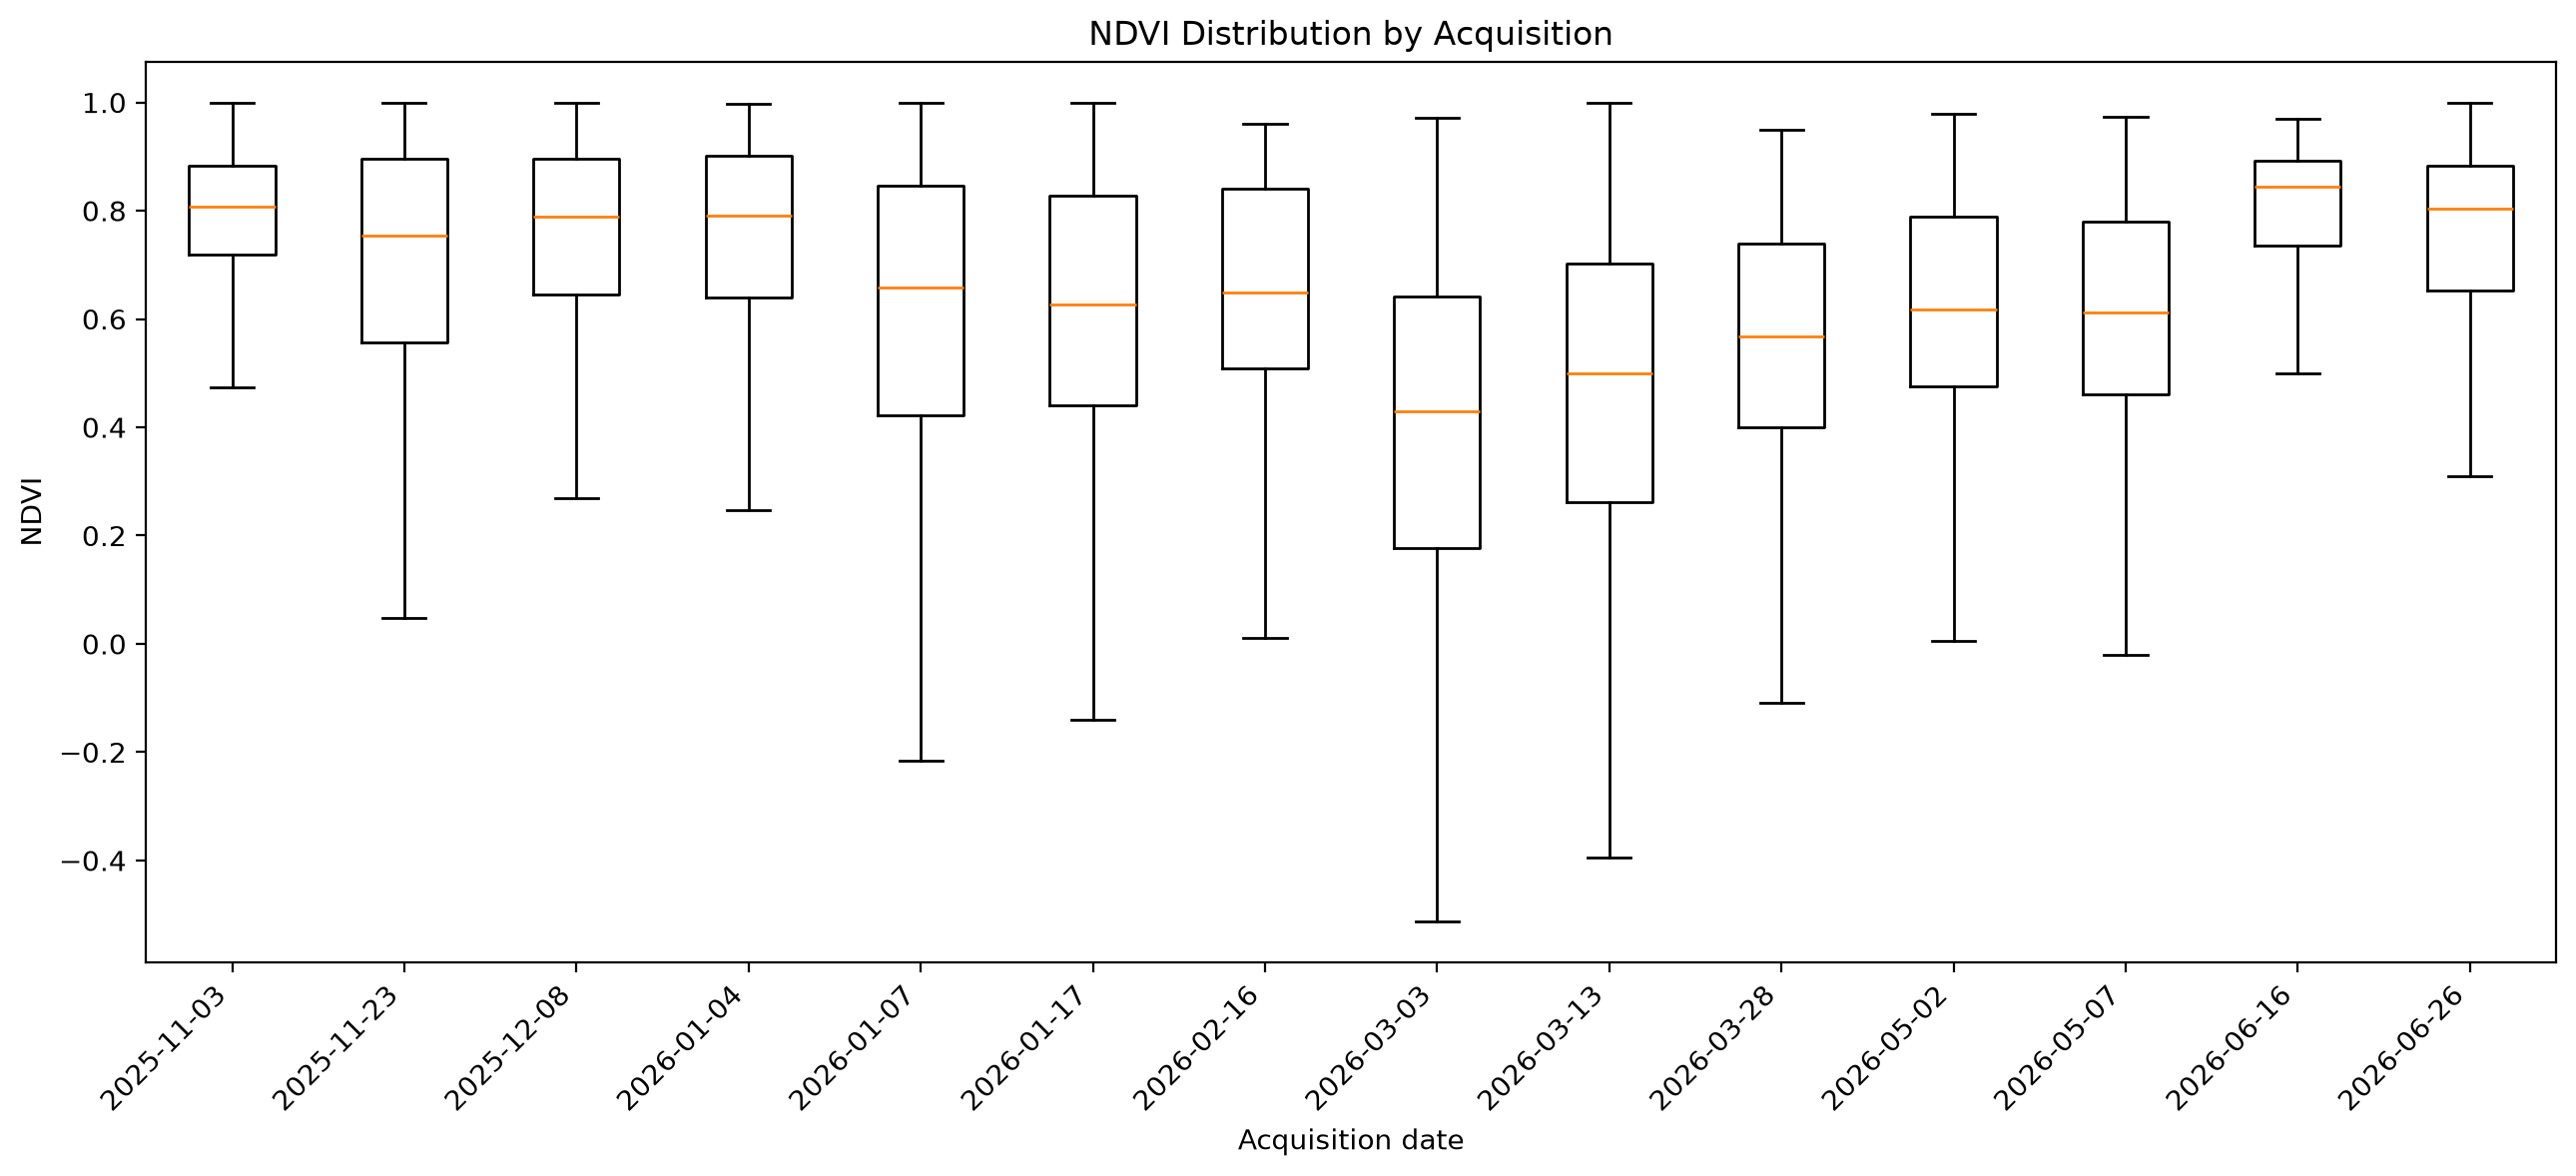
\includegraphics[
	width=0.90\linewidth
	]{../figures/stage5_figure_21.png}
	
	\caption{
		Preliminary distributions of
		pixel-level NDVI values across
		the initially selected
		Sentinel-2 observations.
	}
	
	\label{fig:initial_ndvi_boxplots}
\end{figure}

Inspection revealed that some rasters
provided incomplete spatial coverage
of the broader study area.

The incomplete coverage was associated
with limitations in the available
Sentinel-2 imagery rather than
with the mapped reservoir.

The subsequent agricultural analysis
region was located outside the
affected areas, allowing a consistent
spatial extent to be used for
the final temporal analysis.

The preliminary observations are
therefore presented as exploratory
results and are distinguished from
the final 15-acquisition analysis.


\subsection{Selection of the NDVI Analysis Region}
\label{subsec:ndvi_region_selection}

Five agricultural polygons were selected
from the integrated soil--vegetation
dataset and combined into a unified
analysis region.

Four polygons were associated with
Ferralítico Rojo Típico
(Typical Red Ferrallitic Soil), while
one was associated with
Ferralítico Amarillento Típico
(Typical Yellowish Ferrallitic Soil).

The resulting agricultural analysis
region covered approximately
16.22~km$^2$.

Its spatial distribution is presented
in \Cref{fig:ndvi_selected_region}.

\begin{figure}[htbp]
	\centering
	
	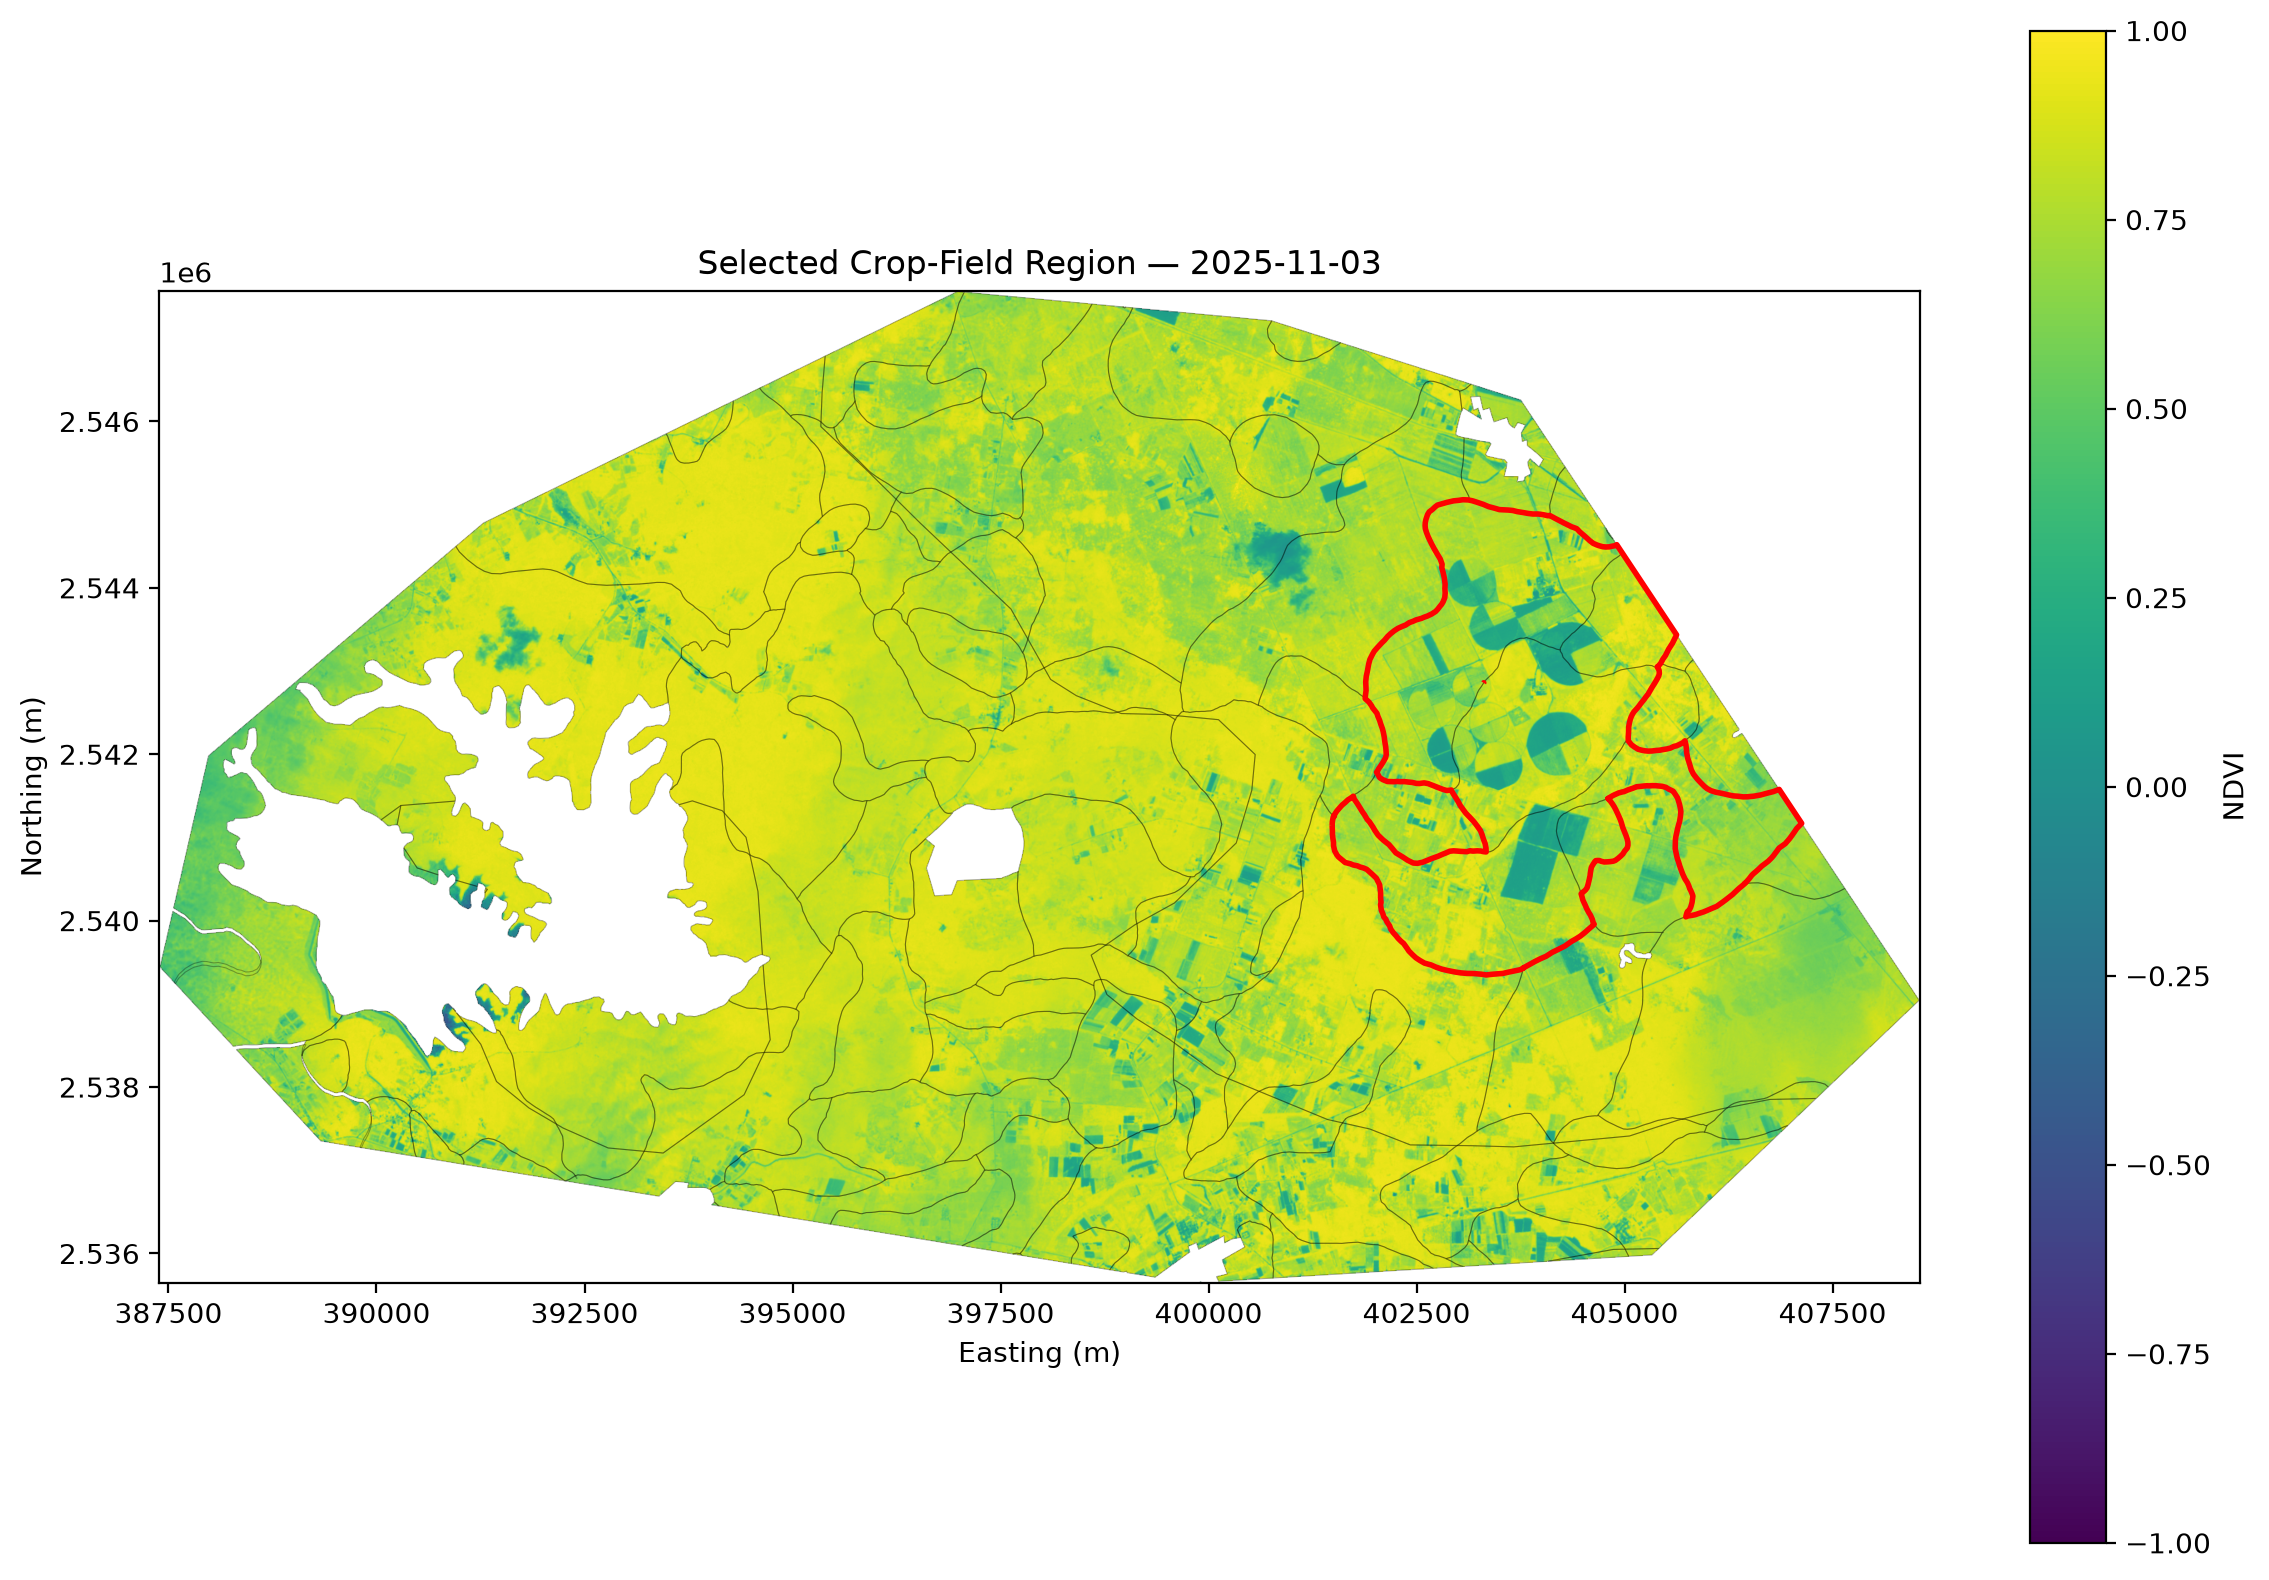
\includegraphics[
	width=0.90\linewidth
	]{../figures/stage5_figure_41.png}
	
	\caption{
		Spatial distribution of the five
		selected agricultural polygons
		and their unified analysis
		region within the study area.
	}
	
	\label{fig:ndvi_selected_region}
\end{figure}

The selected region was located
outside the areas affected by
incomplete satellite coverage
identified during the preliminary
inspection.

The 32 regional NDVI rasters
provided the initial image
collection for this area.

Following regional SCL-based
quality screening, 15 acquisitions
were retained for the temporal
and spatial NDVI analyses.

The retained acquisitions are
illustrated in
\Cref{fig:ndvi_cloud_screening}.

\begin{figure}[htbp]
	\centering
	
	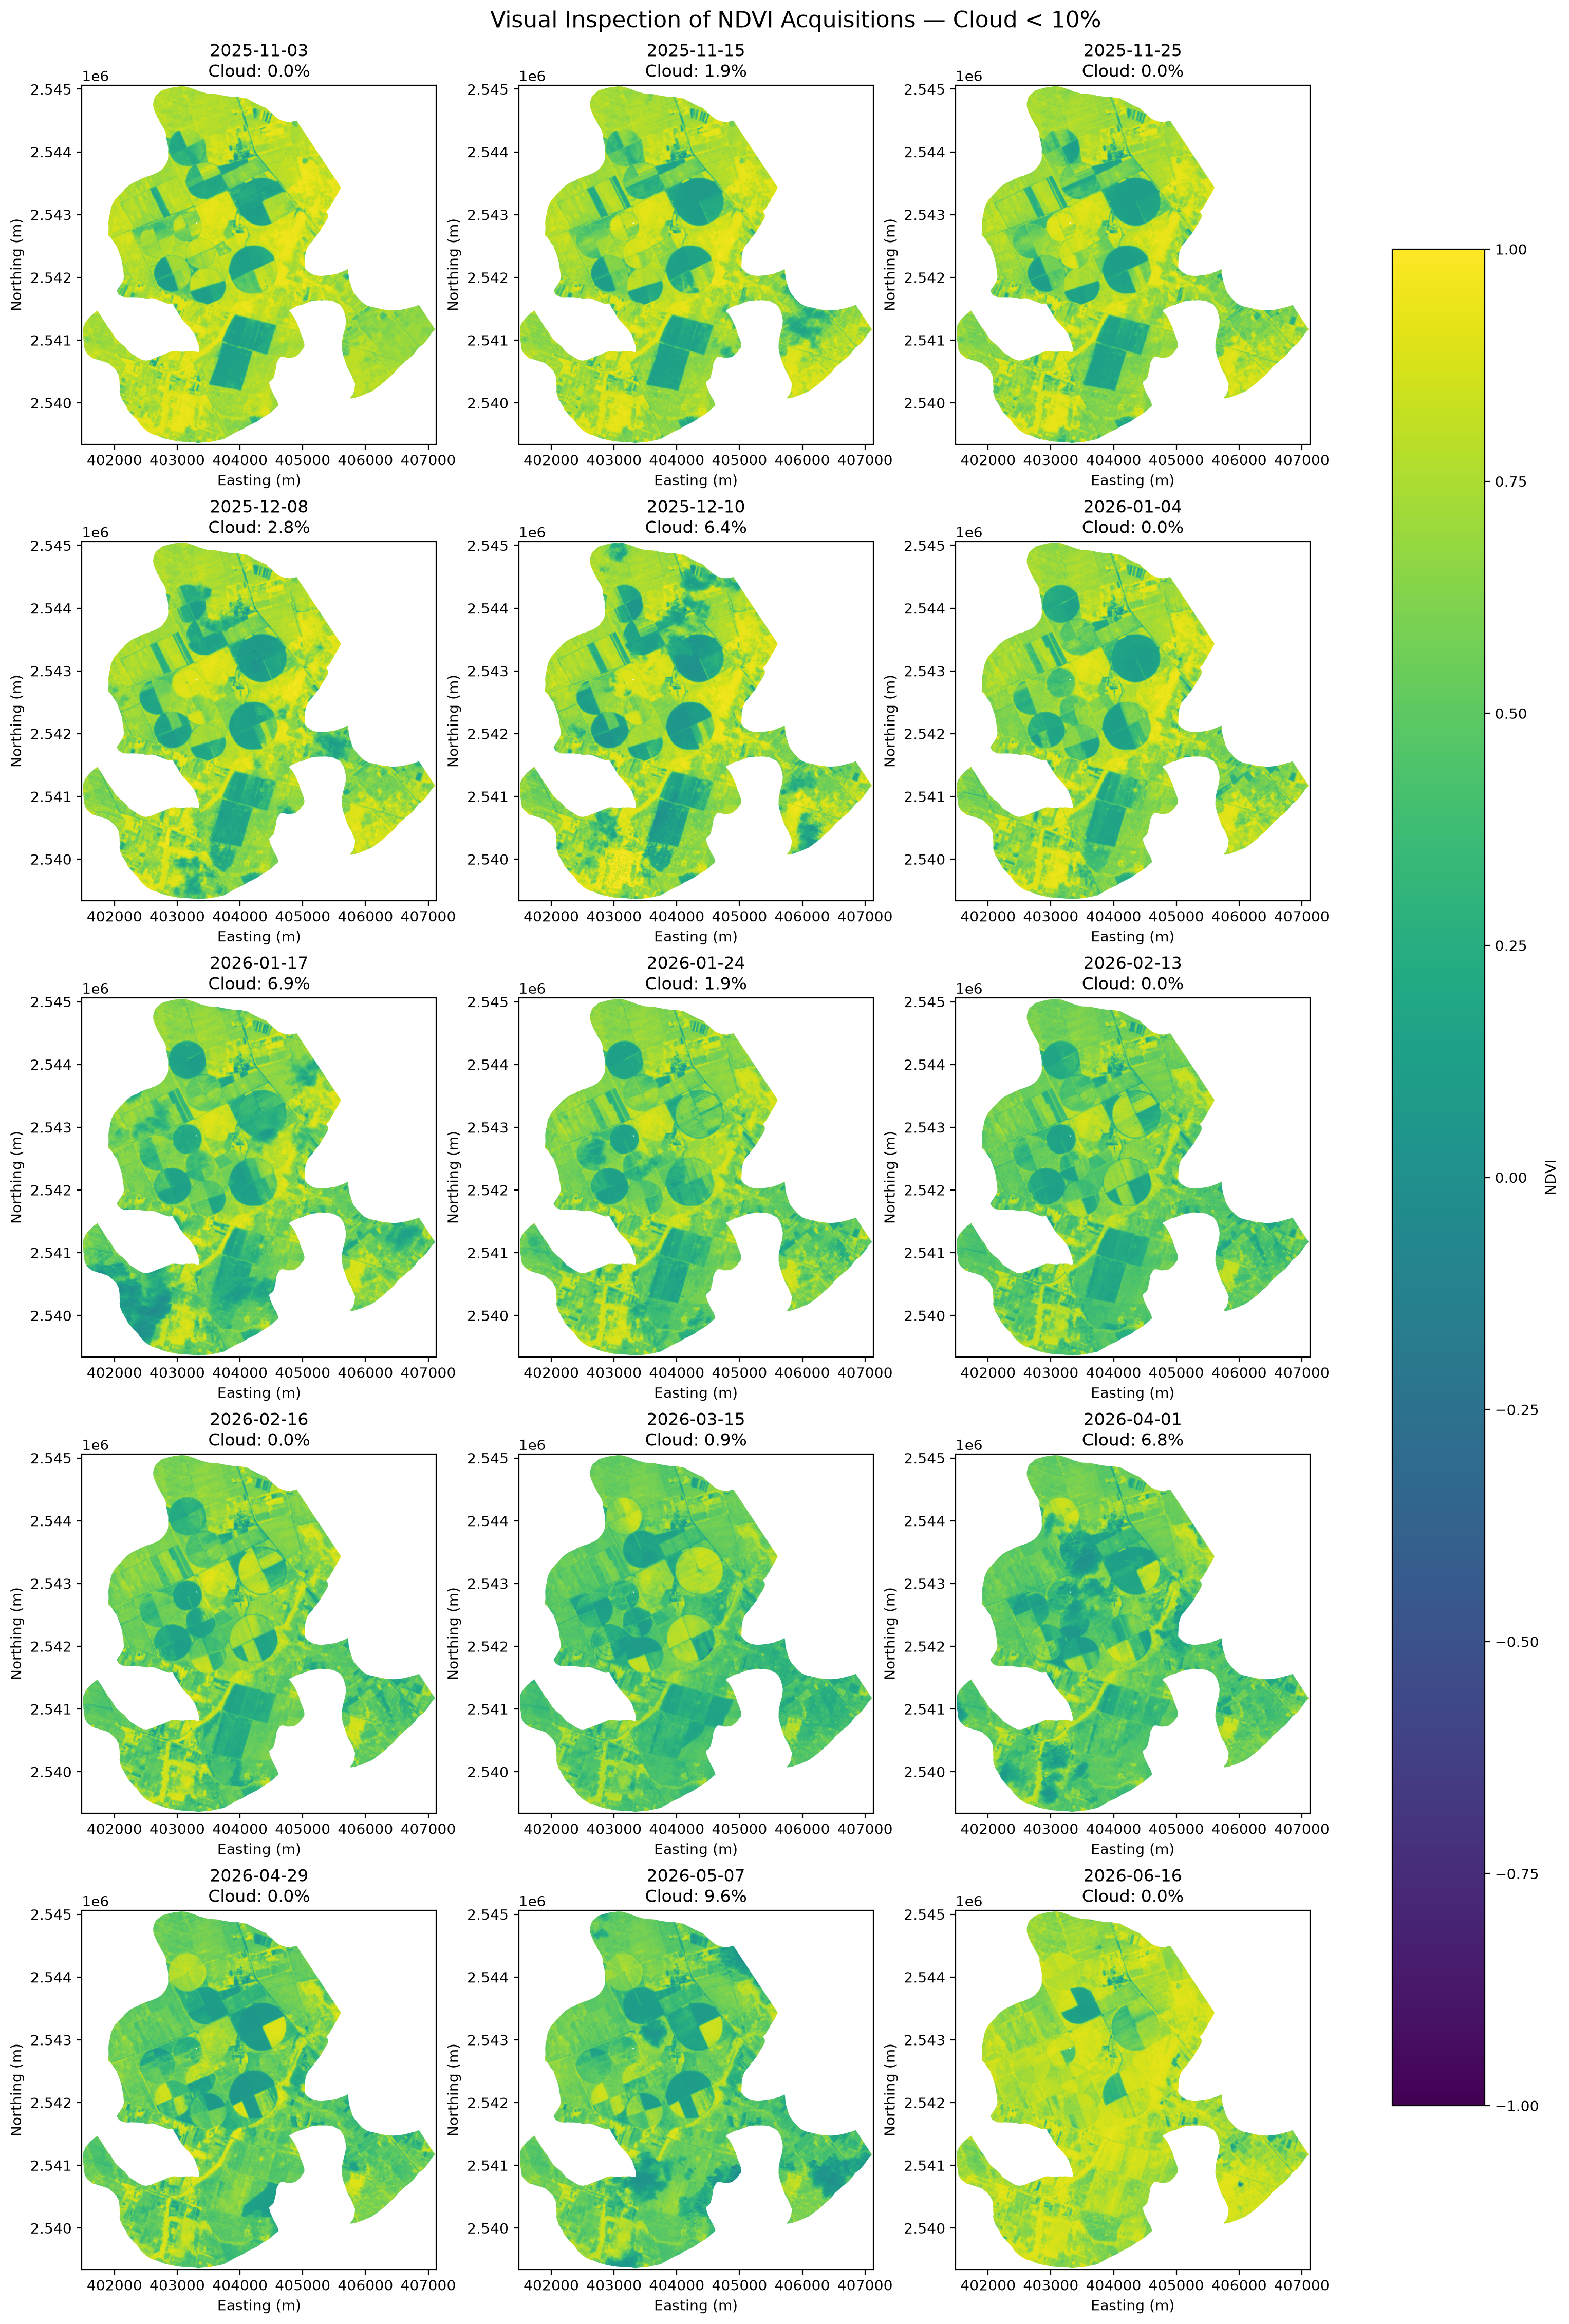
\includegraphics[
	width=\linewidth
	]{../figures/stage5_figure_59.png}
	
	\caption{
		Visual comparison of the
		15 regional NDVI acquisitions
		satisfying the cloud-coverage
		criterion of less than 10\%.
	}
	
	\label{fig:ndvi_cloud_screening}
\end{figure}

The unified region provided a
consistent geographic basis for
comparing vegetation-index
observations throughout the
study period.


\subsection{Temporal NDVI Variability}
\label{subsec:temporal_ndvi_variability}

Temporal NDVI variability was examined
using the mean and median values
calculated for the 15 accepted
Sentinel-2 acquisitions.

The results indicate a general
decline in regional NDVI from
November 2025 through March 2026.

Mean NDVI decreased from approximately
0.688 on 3 November 2025 to
0.466 on 15 March 2026.

Over the same period, median NDVI
declined from approximately
0.754 to 0.463.

Subsequent observations showed
fluctuations rather than a
continuous increase.

Mean NDVI was approximately
0.470 on 1 April 2026,
0.512 on 29 April, and
0.482 on 7 May.

By 16 June 2026, mean NDVI
had increased to approximately
0.737, while median NDVI
reached approximately 0.764.

The temporal evolution of both
statistics is presented in
\Cref{fig:ndvi_temporal_variability}.

\begin{figure}[htbp]
	\centering
	
	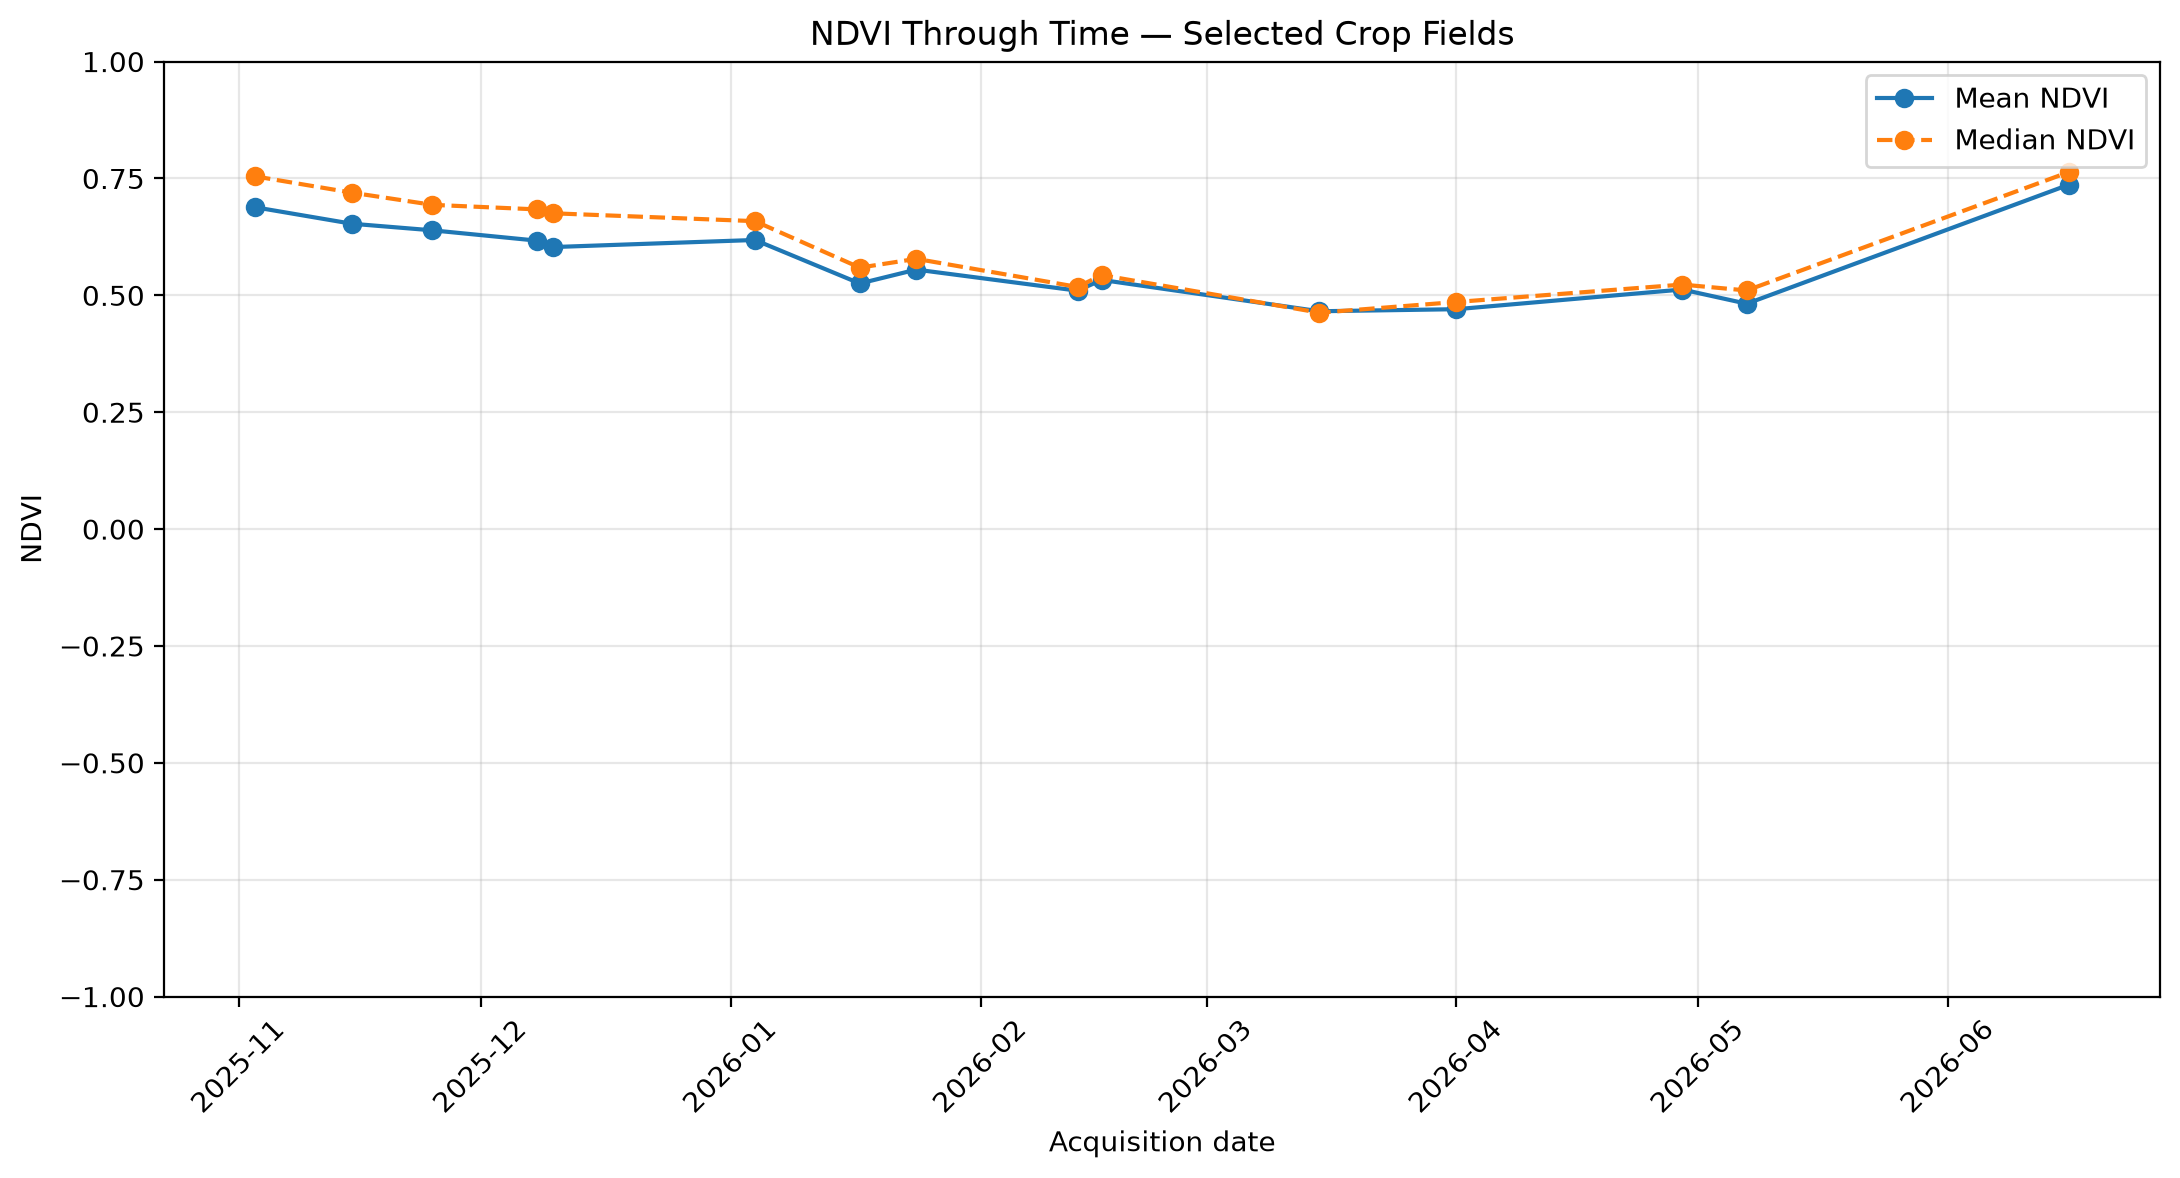
\includegraphics[
	width=0.95\linewidth
	]{../figures/stage5_figure_67.png}
	
	\caption{
		Temporal evolution of mean
		and median NDVI across the
		selected agricultural region
		for the 15 accepted Sentinel-2
		acquisitions from November
		2025 to June 2026.
	}
	
	\label{fig:ndvi_temporal_variability}
\end{figure}

The mean and median series
exhibited broadly similar
temporal patterns.

However, their differences
at individual acquisition dates
indicate that the distributions
were not necessarily symmetric
throughout the observation period.

The regional statistics describe
changes in satellite-derived
vegetation-index values and
do not independently establish
the agricultural or environmental
processes responsible for them.


\subsection{NDVI Distribution and Spatial Variability}
\label{subsec:ndvi_distribution_spatial}

Pixel-level NDVI distributions
were examined to characterize
variability within the selected
agricultural region.

Boxplots for the 15 accepted
acquisitions are presented in
\Cref{fig:ndvi_boxplots}.

\begin{figure}[htbp]
	\centering
	
	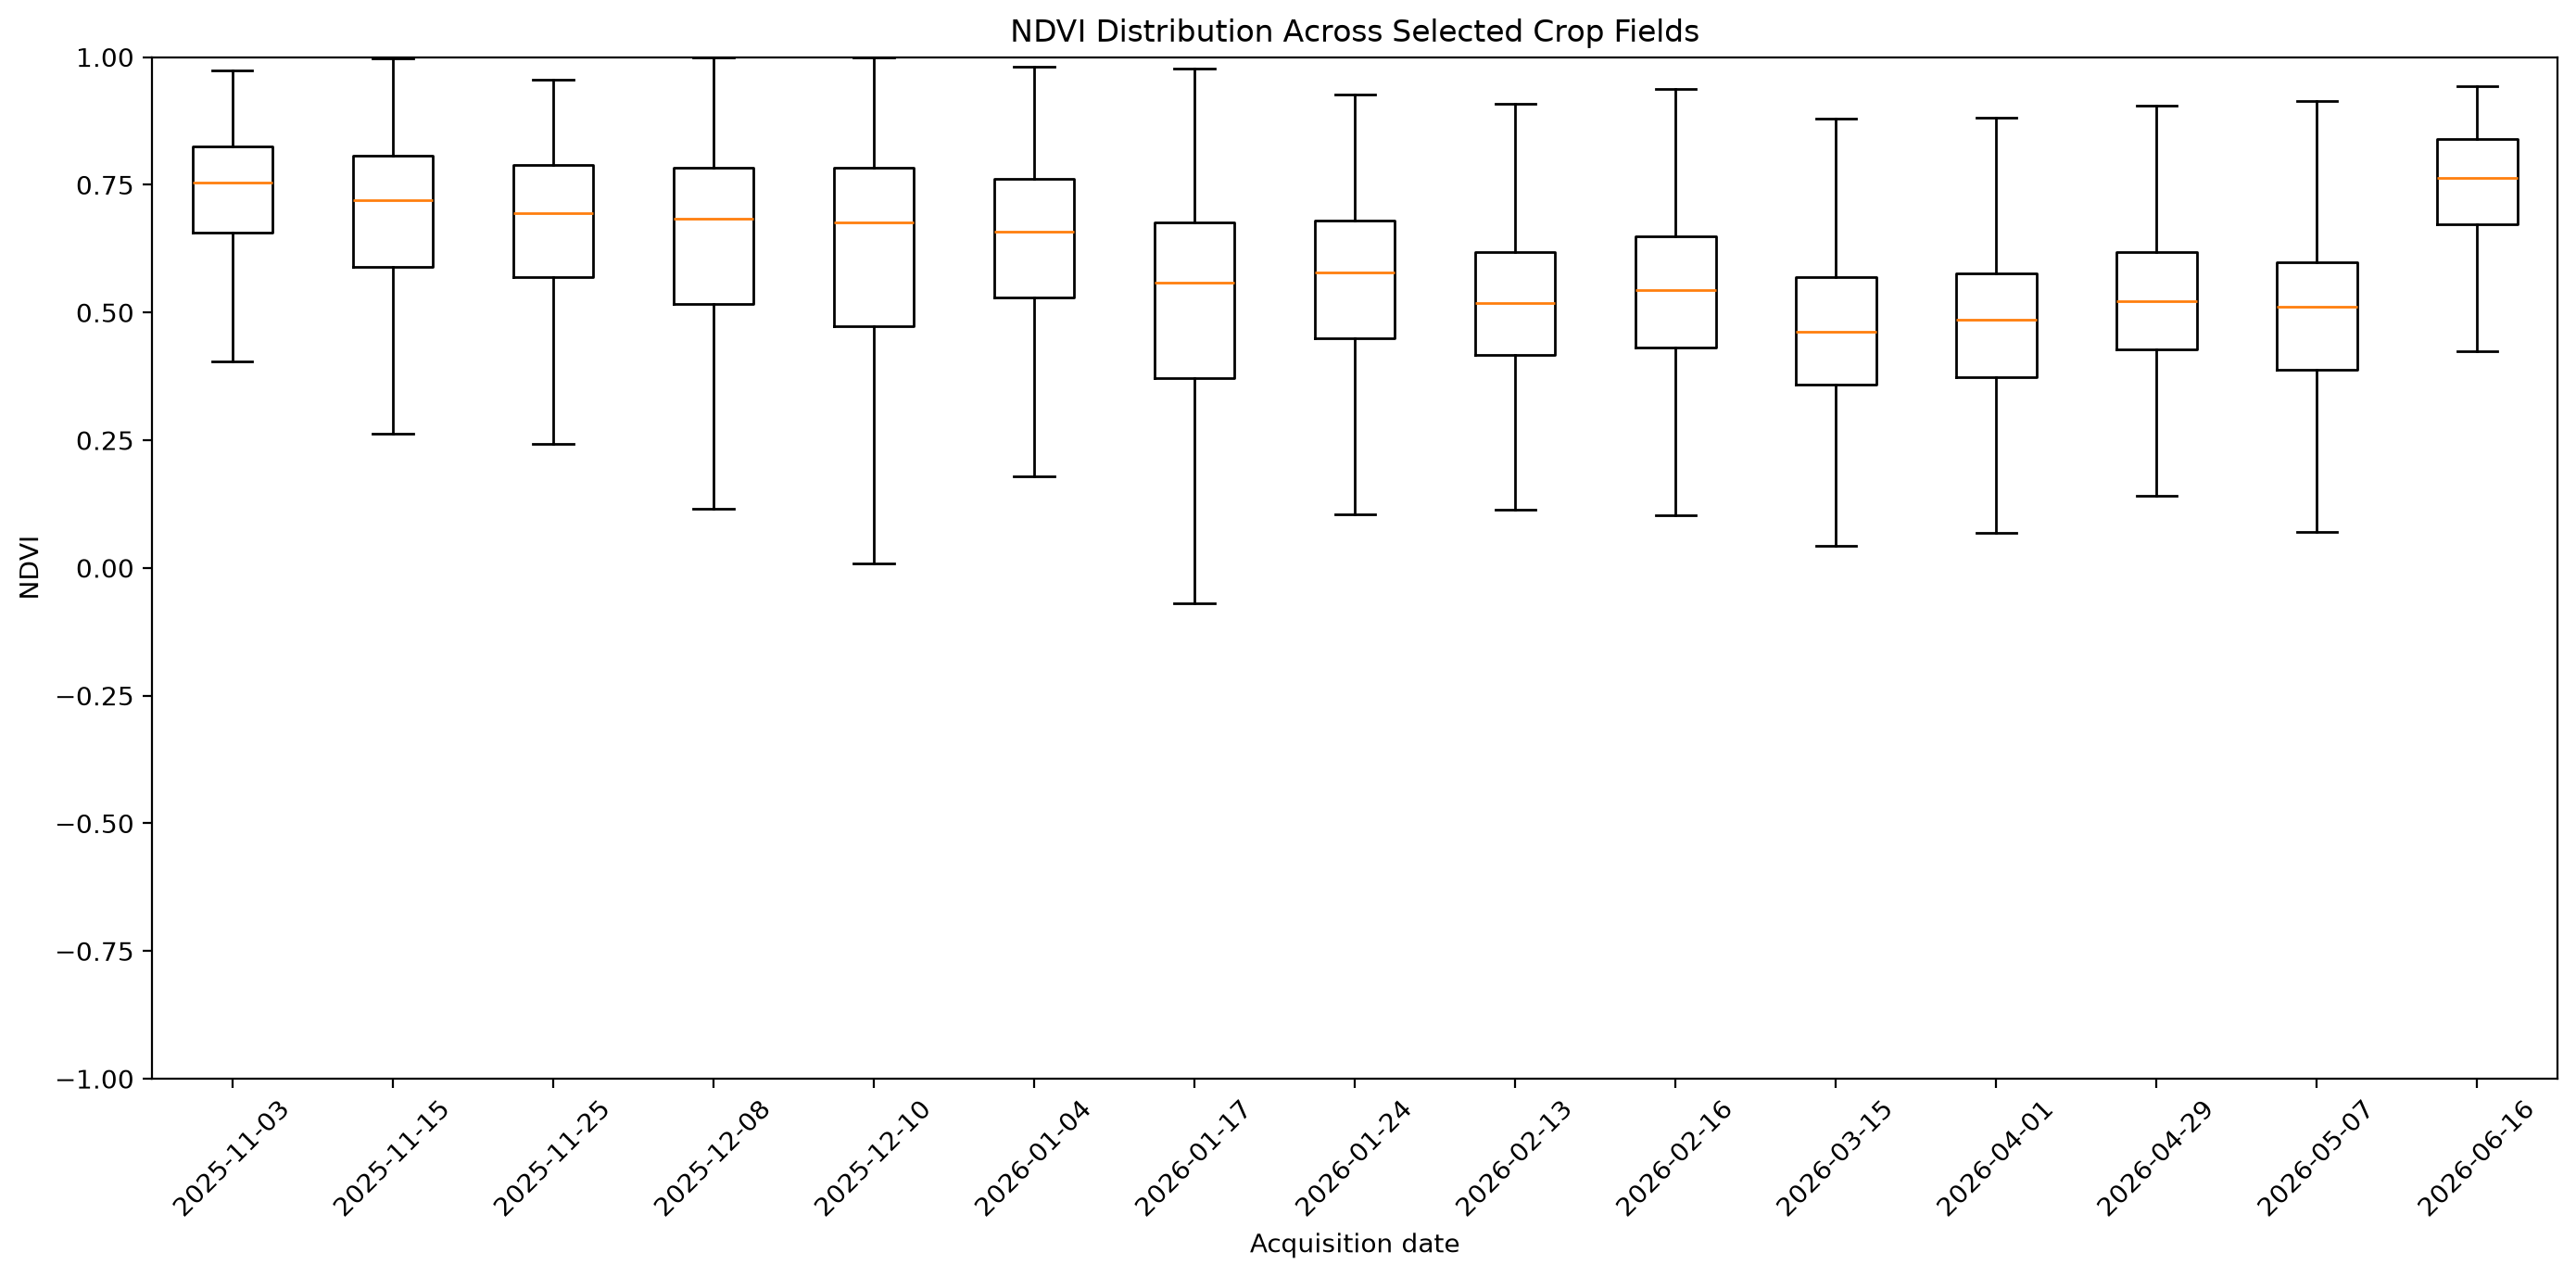
\includegraphics[
	width=0.95\linewidth
	]{../figures/stage5_figure_70.png}
	
	\caption{
		Pixel-level NDVI distributions
		across the 15 accepted
		Sentinel-2 acquisitions,
		represented by boxplots.
	}
	
	\label{fig:ndvi_boxplots}
\end{figure}

The distributions showed changes
in median NDVI, interquartile
range, and overall dispersion
across acquisition dates.

A general shift toward lower
NDVI values was observed between
November 2025 and March 2026,
consistent with the regional
mean and median time series.

To examine differences in
distribution shape, four
representative acquisitions
were selected:

8 December 2025,
16 February 2026,
29 April 2026, and
16 June 2026.

Their NDVI density distributions
are shown in
\Cref{fig:ndvi_density}.

\begin{figure}[htbp]
	\centering
	
	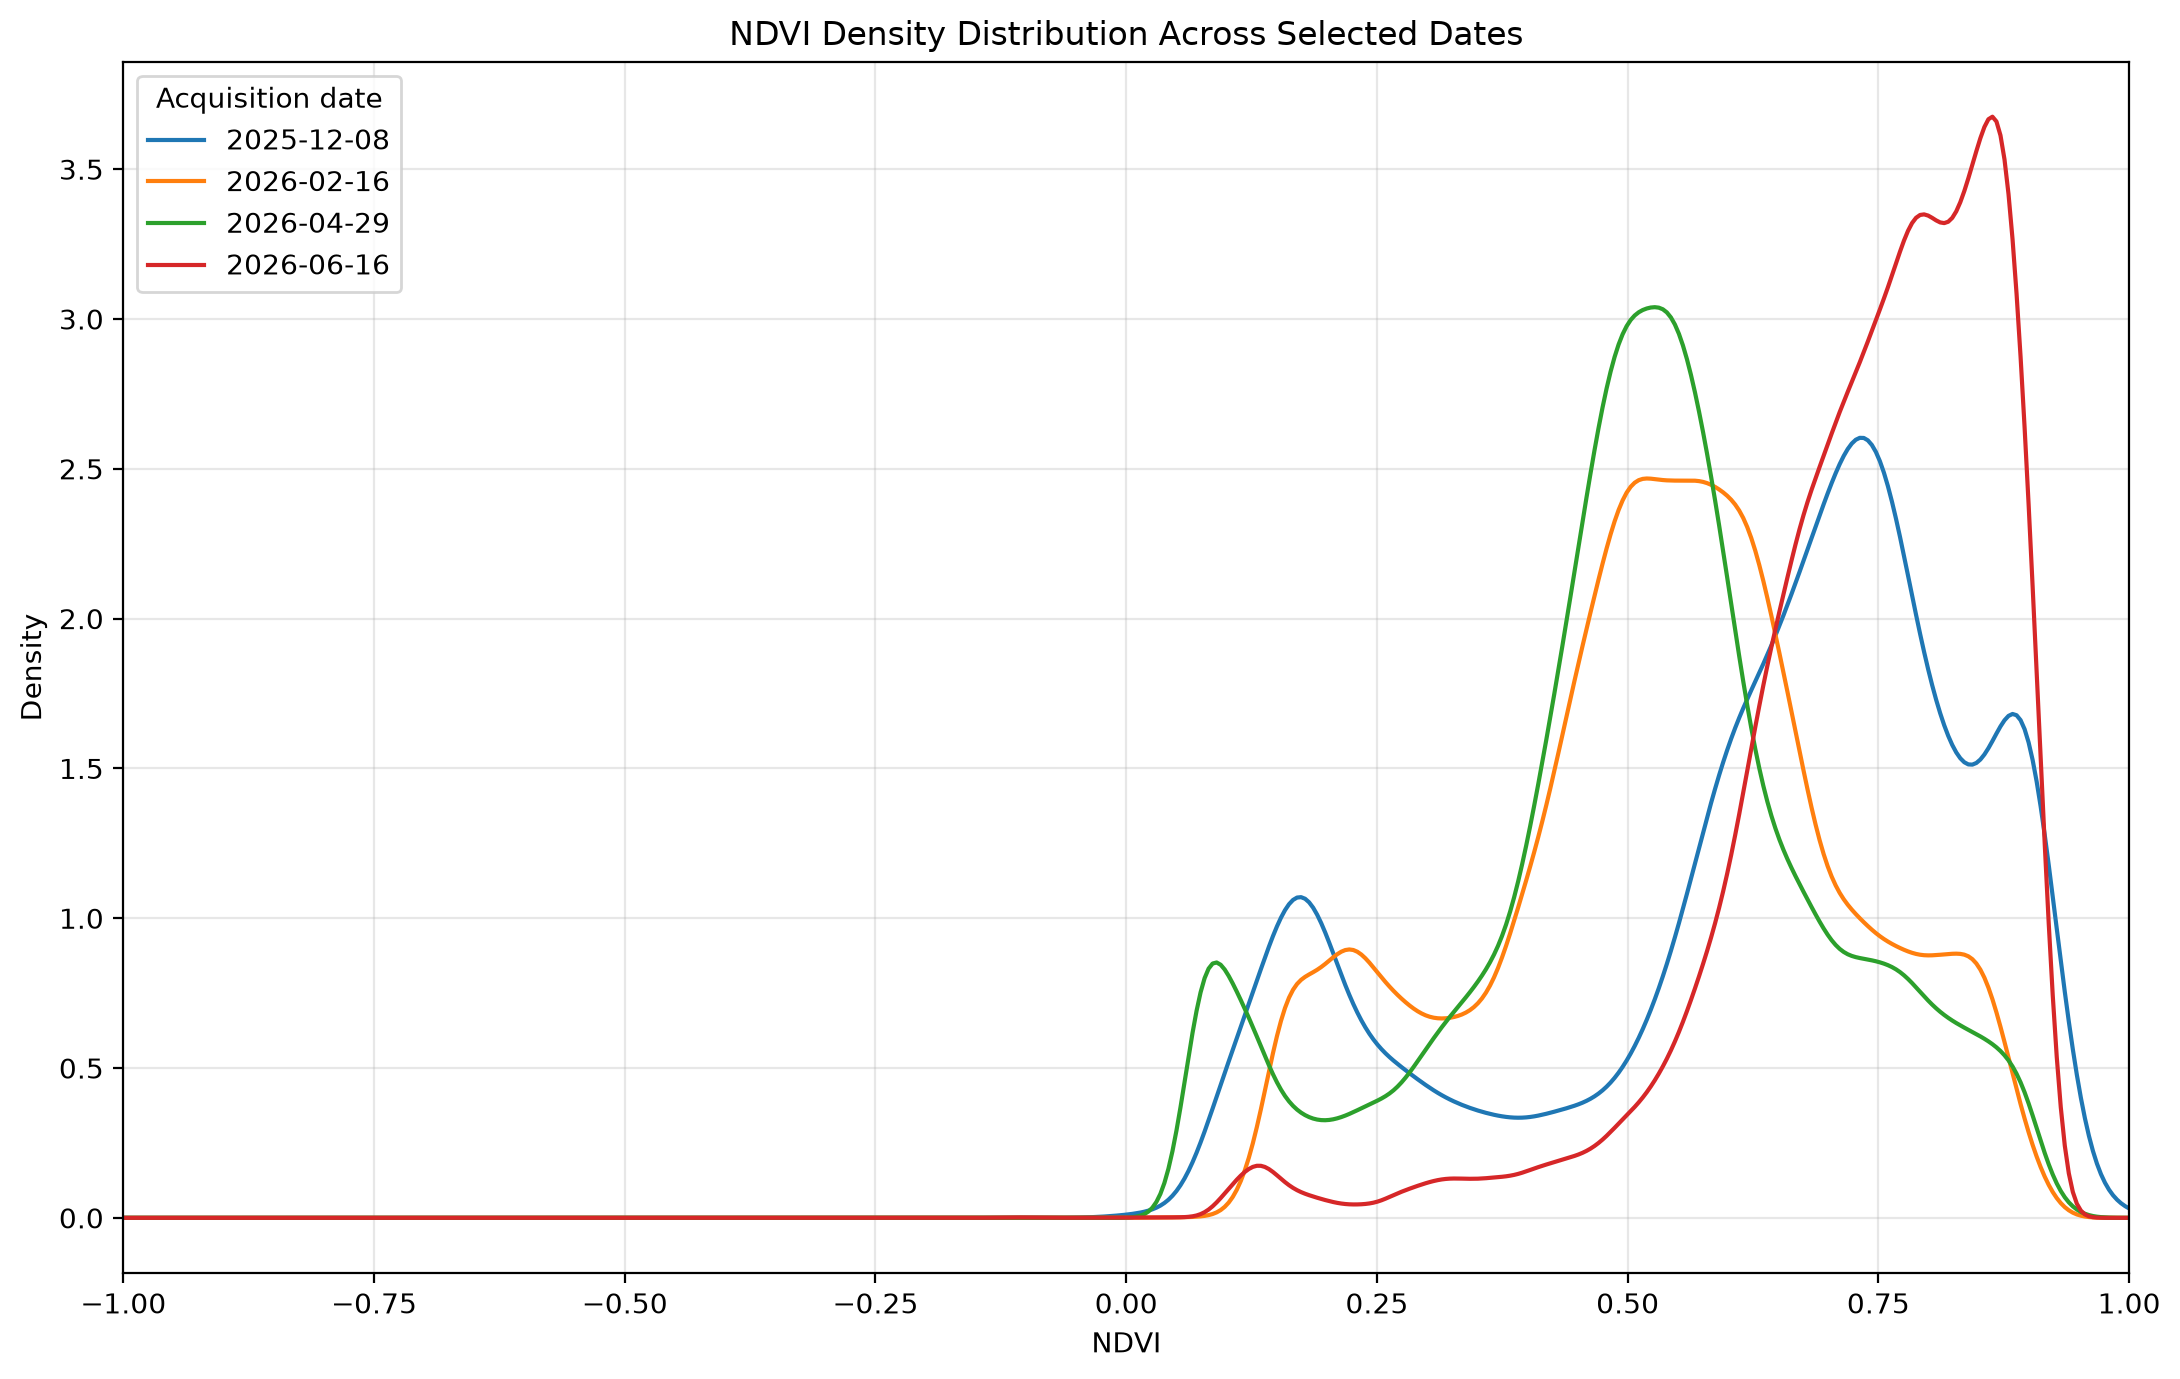
\includegraphics[
	width=0.95\linewidth
	]{../figures/stage5_figure_74.png}
	
	\caption{
		Pixel-level NDVI density
		distributions for four
		representative acquisitions:
		8 December 2025,
		16 February 2026,
		29 April 2026, and
		16 June 2026.
	}
	
	\label{fig:ndvi_density}
\end{figure}

The density curves showed
differences in the relative
frequency of low, intermediate,
and high NDVI values.

These changes indicate that
temporal variability was not
limited to shifts in the
regional mean.

The spatial distribution of
NDVI was also examined for
the same four acquisitions,
as shown in
\Cref{fig:ndvi_spatial_maps}.

\begin{figure}[htbp]
	\centering
	
	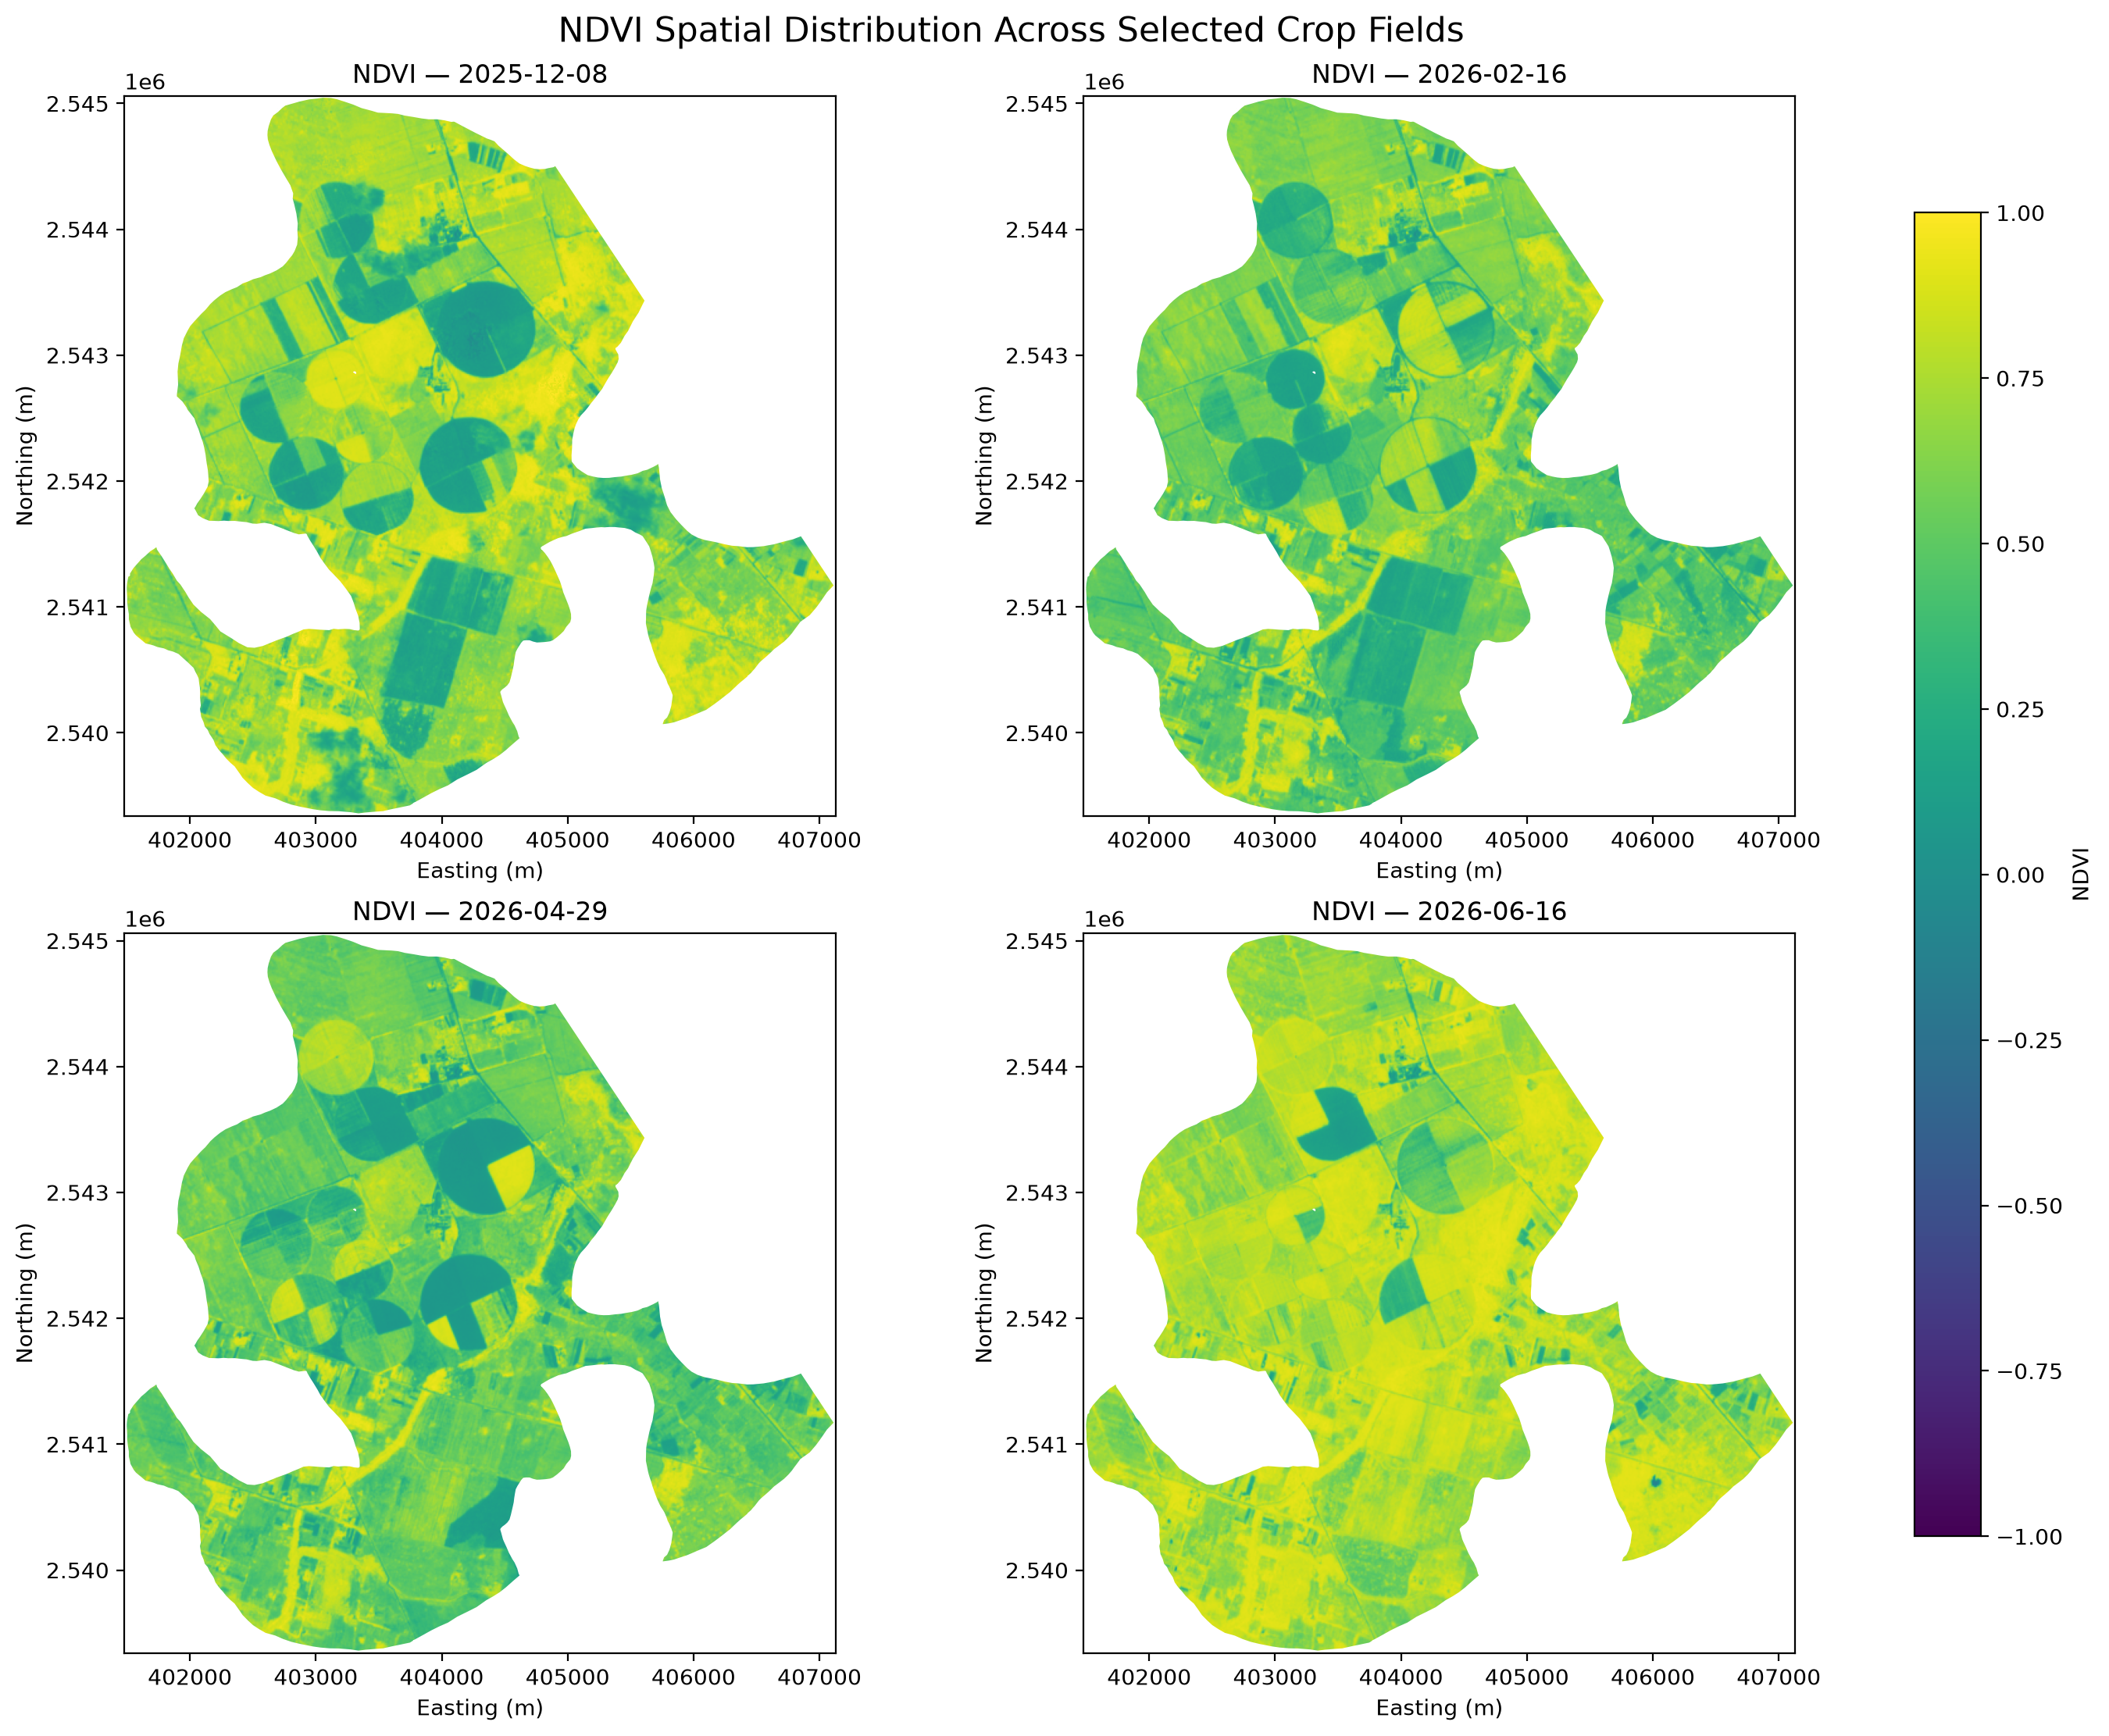
\includegraphics[
	width=\linewidth
	]{../figures/stage5_figure_76.png}
	
	\caption{
		Spatial distribution of
		NDVI within the selected
		agricultural region on
		8 December 2025,
		16 February 2026,
		29 April 2026, and
		16 June 2026.
		All panels use the same
		NDVI scale.
	}
	
	\label{fig:ndvi_spatial_maps}
\end{figure}

The maps revealed geographic
differences in NDVI within
the agricultural region.

Relatively high and low
vegetation-index values were
not distributed uniformly
across the selected polygons.

The June observation exhibited
higher regional NDVI values
than those recorded during
March and April.

However, these regional
distributions include multiple
agricultural and vegetation
conditions and cannot be
interpreted as observations
of potato cultivation alone.


\subsection{Field-Level NDVI Analysis of Selected Potato Fields}
\label{subsec:potato_field_analysis}

A complementary field-level
analysis examined three
locally verified potato fields
within the agricultural region.

The fields were represented
by circular sampling polygons
digitized in QGIS.

Their locations and the
sampling configuration are
illustrated in
\Cref{fig:potato_field_selection}.

\begin{figure}[htbp]
	\centering
	
	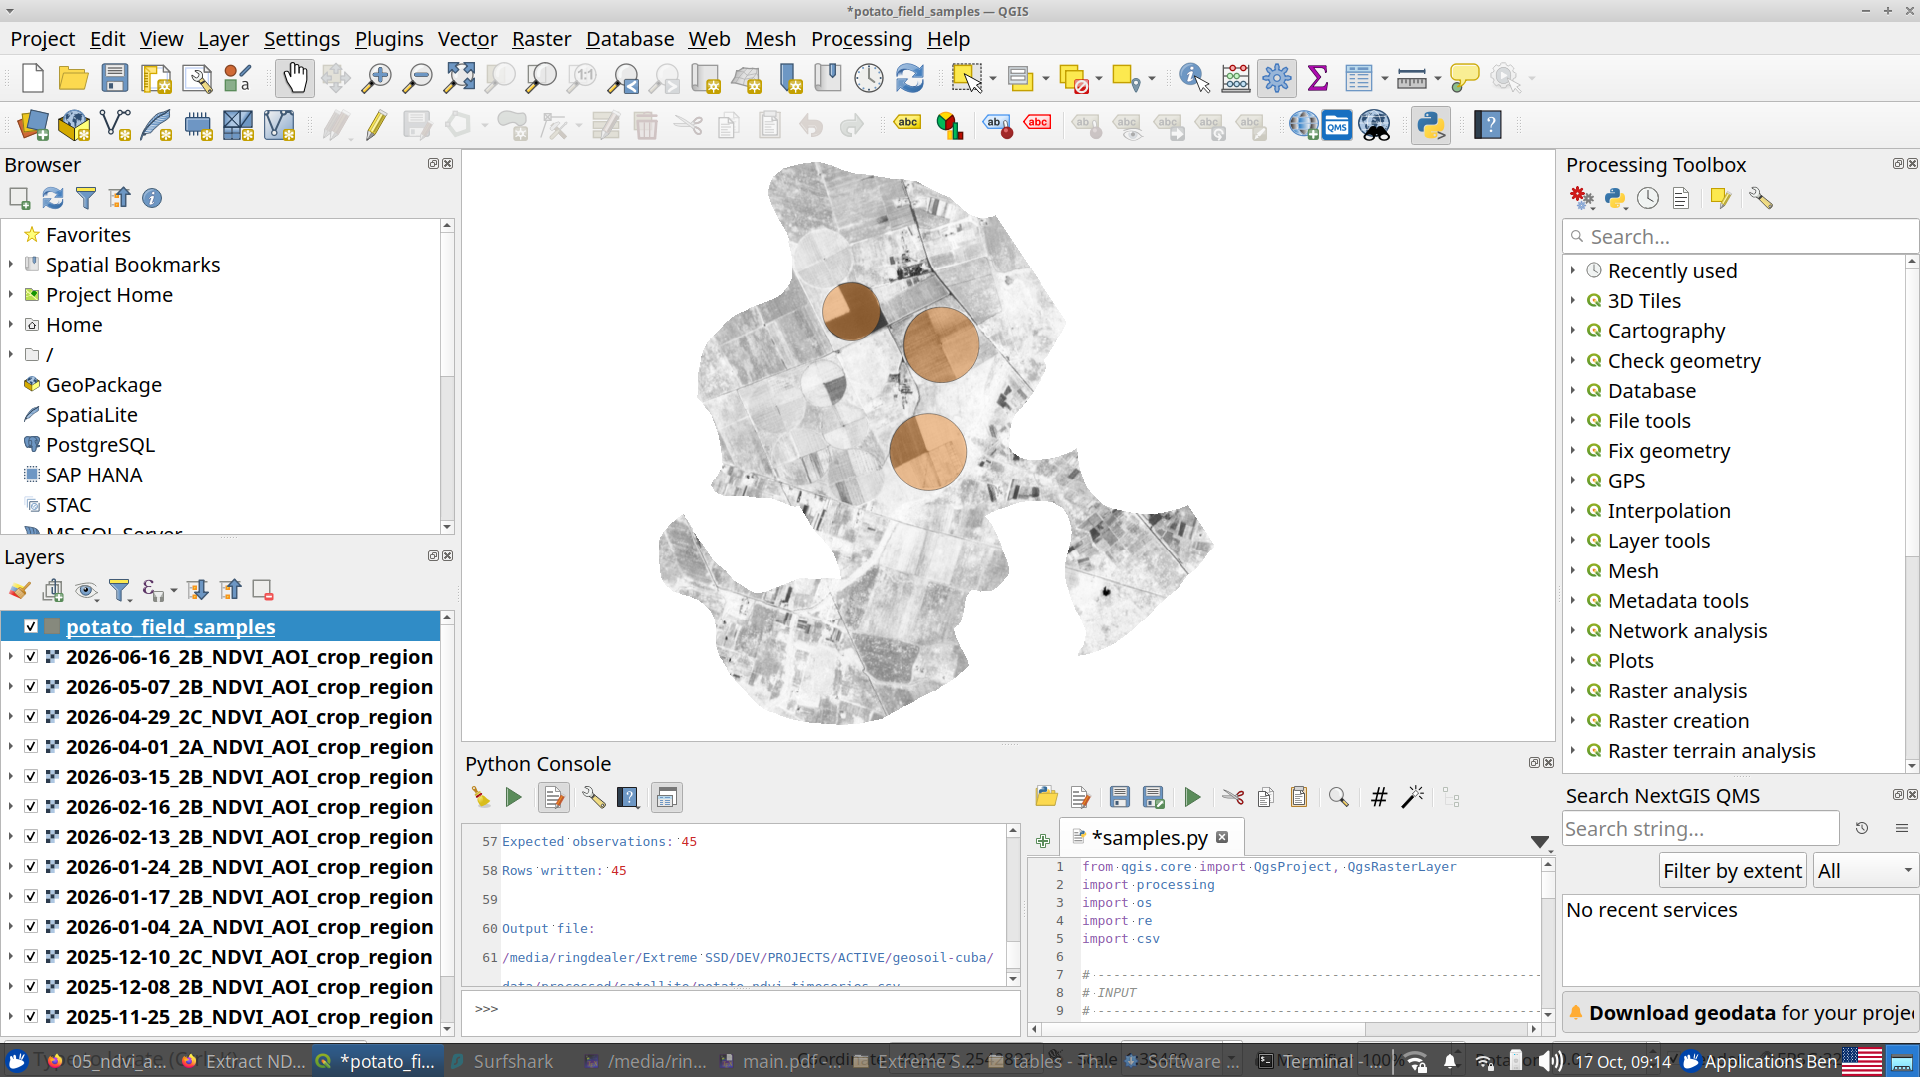
\includegraphics[
	width=\linewidth
	]{../figures/potato_samples.png}
	
	\caption{
		Three locally verified
		potato-field sampling areas
		digitized in QGIS and
		displayed over the
		agricultural-region
		NDVI raster.
	}
	
	\label{fig:potato_field_selection}
\end{figure}

NDVI observations were extracted
for each sampling polygon across
the 15 accepted acquisition dates,
yielding 45 field-date observations.

The number of valid pixels
differed among the sampling
polygons but remained constant
across the acquisition dates
for each field.

Field 1 contained 4,603 valid
pixels, Field 2 contained
4,785 pixels, and Field 3
contained 2,710 pixels.

The temporal evolution of
mean NDVI for the three fields
is presented in
\Cref{fig:potato_field_timeseries}.

\begin{figure}[htbp]
	\centering
	
	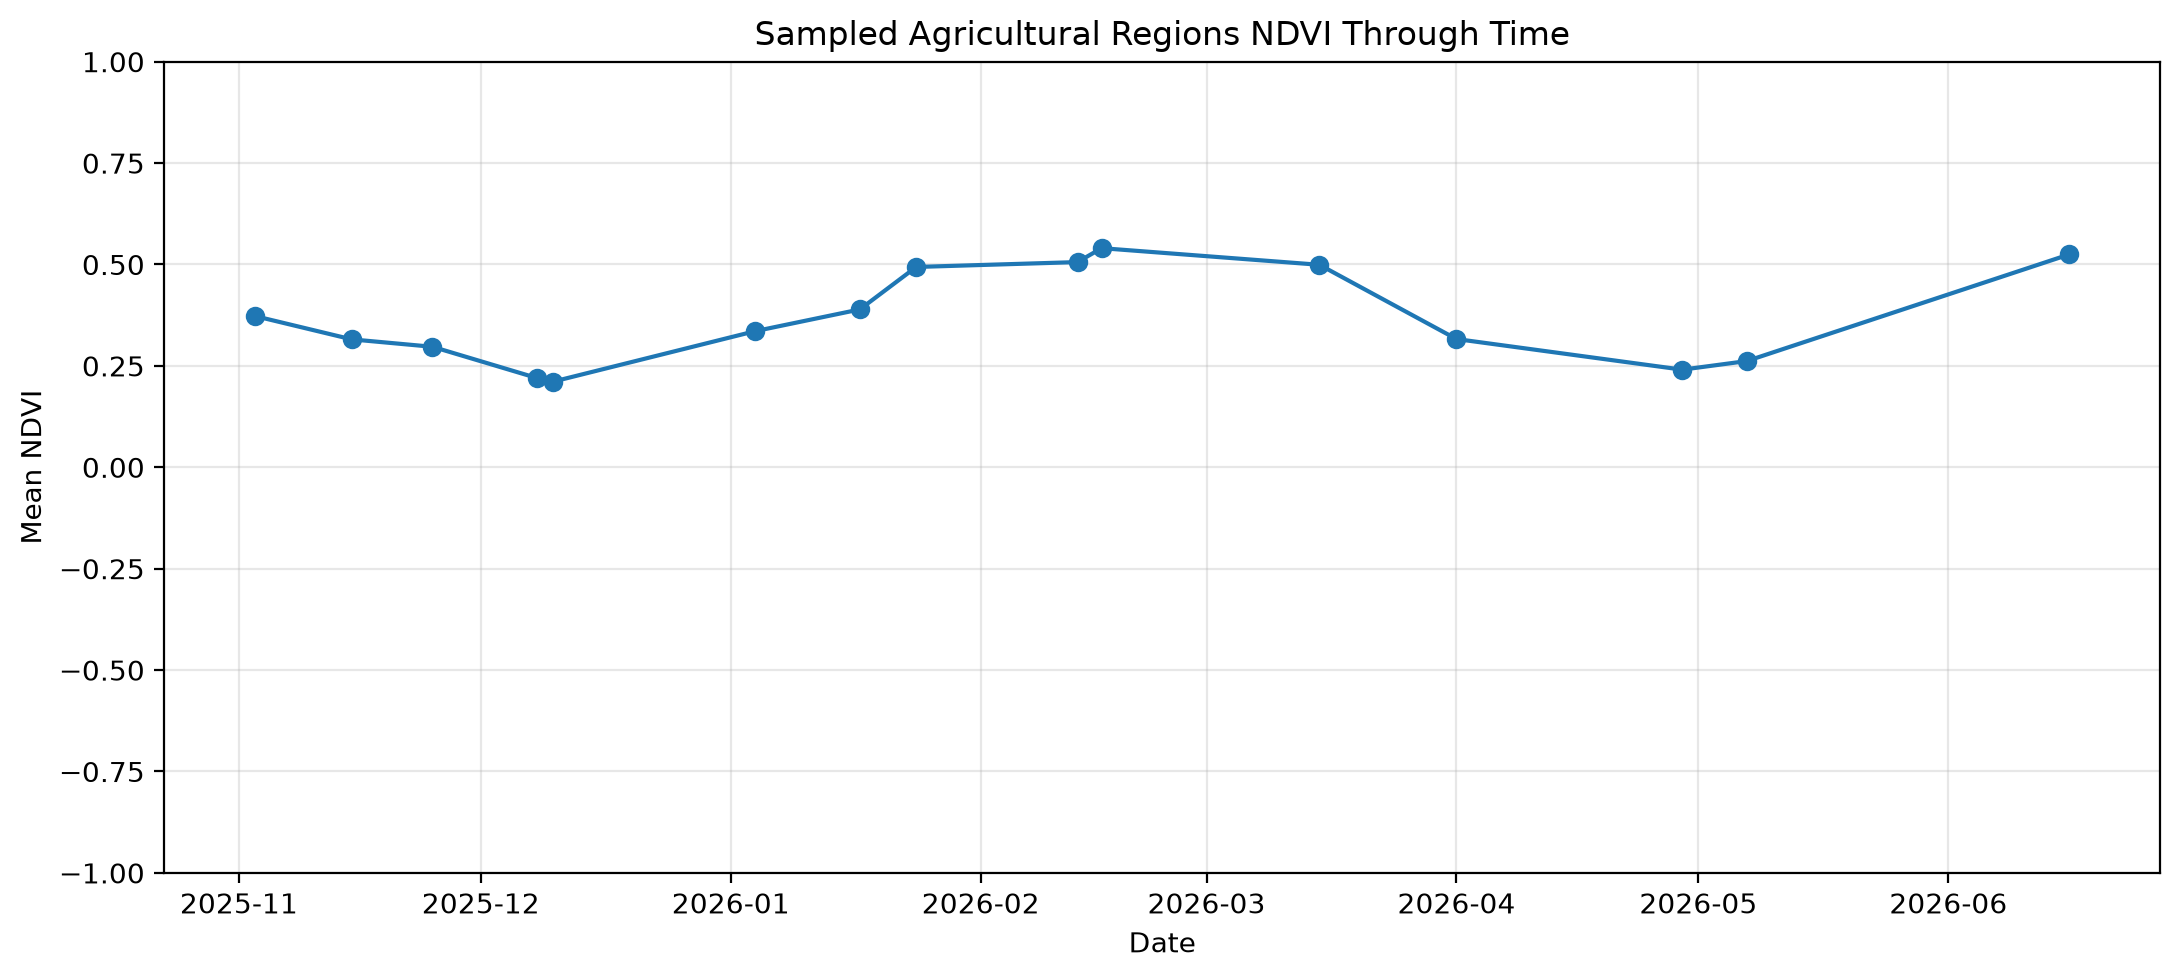
\includegraphics[
	width=0.95\linewidth
	]{../figures/stage5_figure_84.png}
	
	\caption{
		Temporal evolution of
		mean NDVI across the
		three selected potato-field
		sampling areas from
		November 2025 to June 2026.
	}
	
	\label{fig:potato_field_timeseries}
\end{figure}

The three sampled areas exhibited
different temporal NDVI patterns.

Field 1 reached its highest
mean NDVI of approximately
0.744 on 15 March 2026.

Field 2 reached its highest
mean NDVI of approximately
0.690 on 16 June 2026.

Field 3 reached its highest
mean NDVI of approximately
0.573 on 24 January 2026,
followed by a substantial
decline in subsequent
observations.

The maximum observed mean NDVI
values and their corresponding
dates are summarized in
\Cref{tab:potato_field_maxima}.

\begin{table}[htbp]
	\centering
	
	\caption{
		Maximum observed mean NDVI
		for the three selected
		potato-field sampling areas.
	}
	
	\label{tab:potato_field_maxima}
	
	\begin{tabular}{lcc}
		\hline
		
		\textbf{Field} &
		\textbf{Maximum mean NDVI} &
		\textbf{Acquisition date} \\
		
		\hline
		
		Field 1 & 0.744 & 15 March 2026 \\
		Field 2 & 0.690 & 16 June 2026 \\
		Field 3 & 0.573 & 24 January 2026 \\
		
		\hline
	\end{tabular}
\end{table}

The different dates of
maximum mean NDVI indicate
that the sampled fields
did not follow identical
vegetation-index trajectories.

Pixel-level NDVI distributions
were also examined using
boxplots, as presented in
\Cref{fig:potato_field_boxplots}.

\begin{figure}[htbp]
	\centering
	
	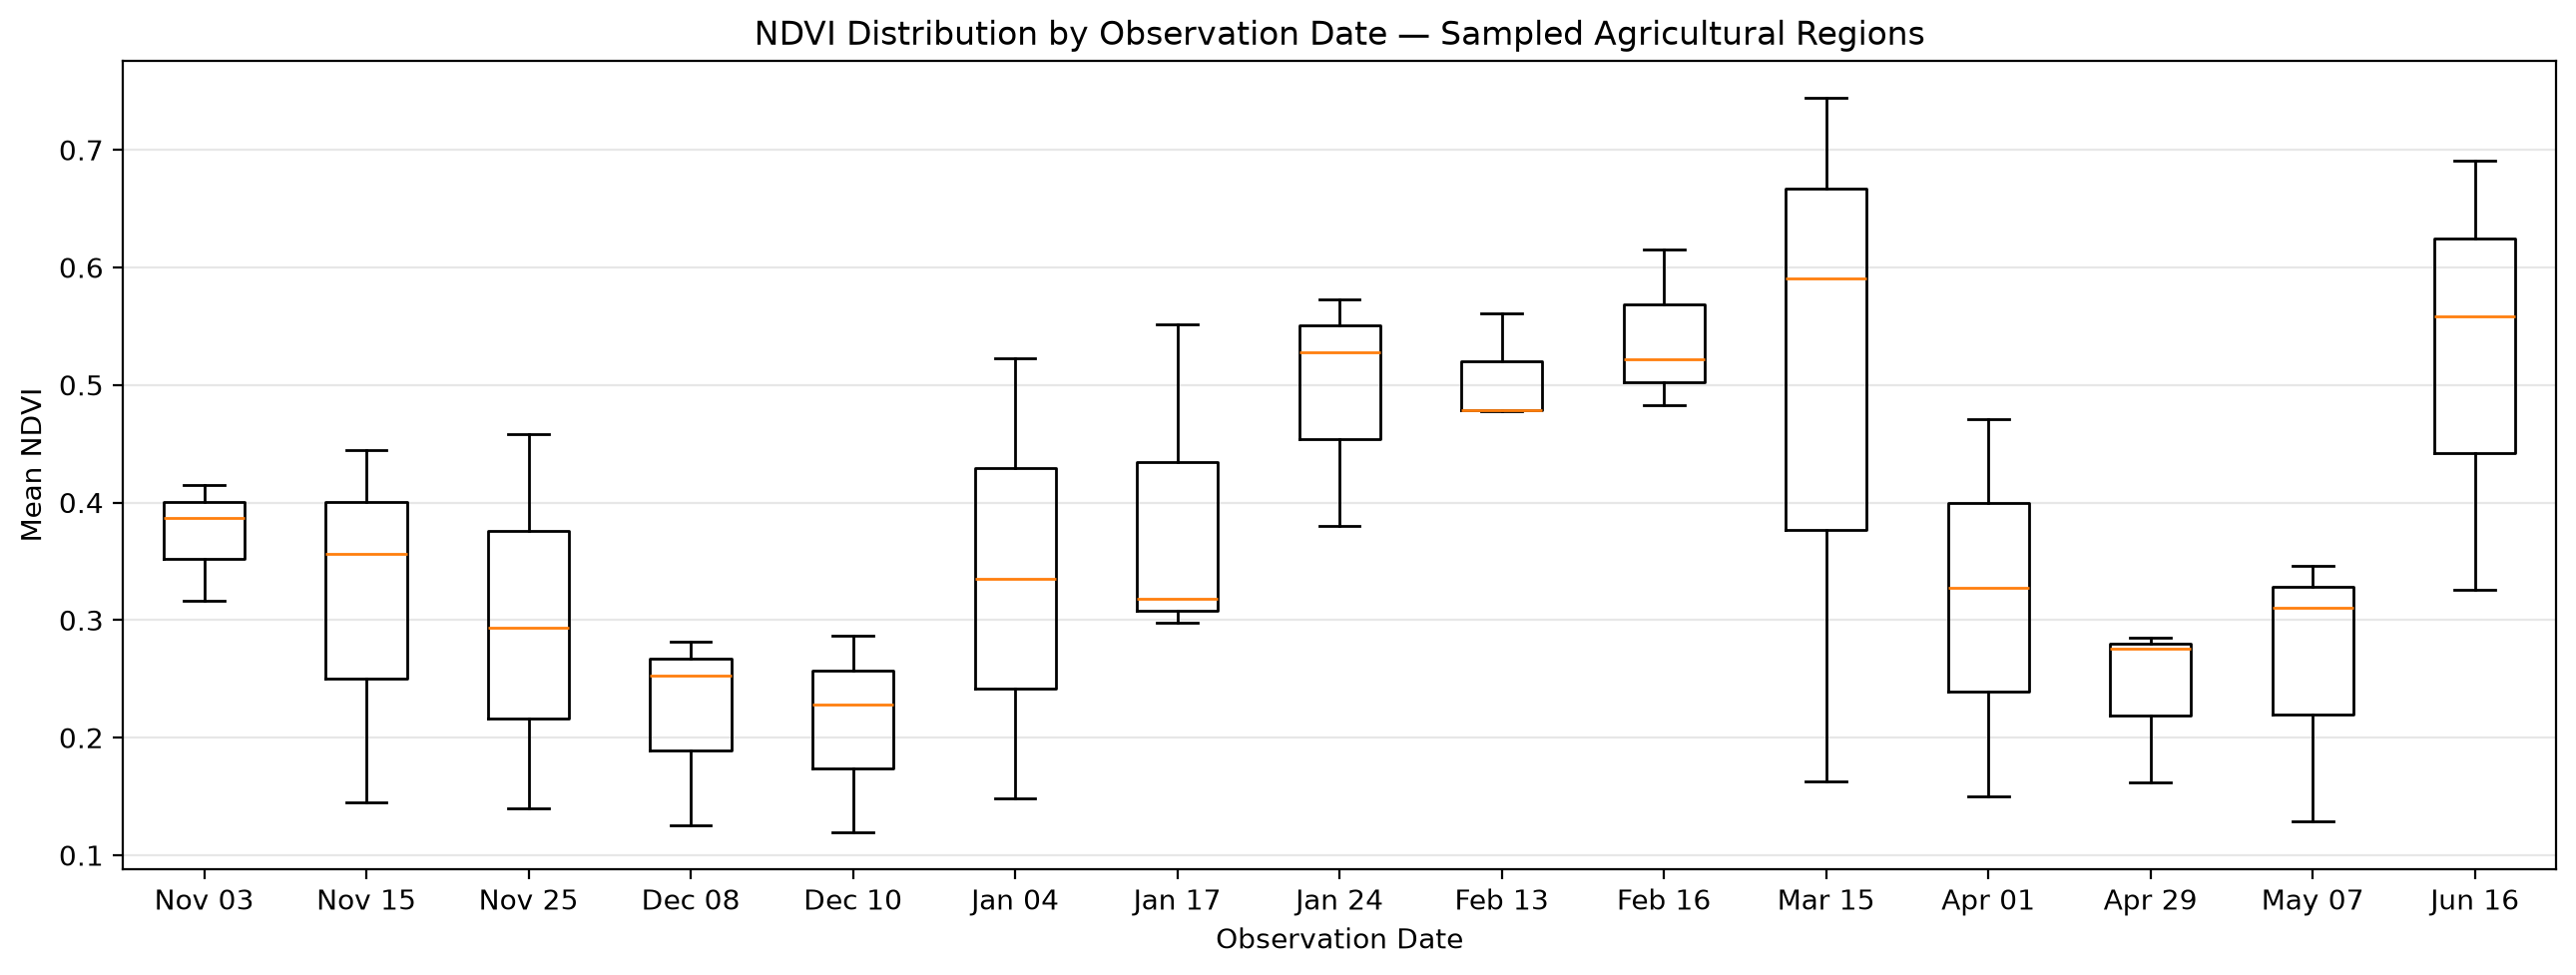
\includegraphics[
	width=0.95\linewidth
	]{../figures/stage5_figure_86}
	
	\caption{
		Distribution of NDVI
		observations across the
		three selected potato-field
		sampling areas and
		acquisition dates.
	}
	
	\label{fig:potato_field_boxplots}
\end{figure}

The field-level results
demonstrate temporal variability
within the selected agricultural
sampling areas that is not
fully represented by the
regional mean NDVI series.

The observed differences
provide a basis for further
investigation of agricultural
conditions but do not
independently identify
crop-development stages,
harvesting dates, or
management practices.